\documentclass{patmorin}
\usepackage[utf8]{inputenc}
\usepackage{amsthm,amsmath,graphicx}
\usepackage{array}
\usepackage{pat}
\usepackage{hyperref}
\usepackage[dvipsnames]{xcolor}
\definecolor{linkblue}{named}{Blue}
\hypersetup{colorlinks=true, linkcolor=linkblue,  anchorcolor=linkblue,
citecolor=linkblue, filecolor=linkblue, menucolor=linkblue,
urlcolor=linkblue, pdfcreator=Me, pdfproducer=Me} \setlength{\parskip}{1ex}
\usepackage{tikz}

\usepackage{paralist}

\DeclareMathOperator{\sgn}{sgn}

\newtheorem{definition}{Definition}
%\newtheorem{proposition}{Proposition}

\newcommand{\Fary}{Fáry}

\listfiles
\newcommand{\lstlabel}[1]{\label{lst:#1}}
\newcommand{\lstref}[1]{Listing~\ref{lst:#1}}
\newcommand{\Lstref}[1]{\lstref{#1}}

\DeclareMathOperator{\block}{block}
\newcommand{\naive}{na\"{\i}ve}


\newcommand{\reals}{\mathbb{R}}
\newcommand{\integers}{\mathbb{Z}}
\newcommand{\naturals}{\mathbb{N}}
\newcommand{\dist}{{d}}

\title{\MakeUppercase{Every Collinear Set is Free}}

\author{Vida Dujmović, Fabrizio Frati, Daniel Gonçalves, Pat Morin, and Günter Rote}

\begin{document}
\maketitle


\begin{abstract}
  We show that if a planar graph $G$ has a plane straight-line embedding
  in which a subset $S$ of its vertices are collinear, then for any set
  $X\subset\R^2$ with $|X|=|S|$ points, there is a plane straight-line
  embedding of $G$ in which the vertices in $S$ are mapped to the points
  in $X$.  This solves an open problem posed by Ravsky and Verbitsky in
  2008.  In their terminology, we show that every collinear set is free.
  This result has applications in graph drawing, including untangling,
  column planarity, universal point subsets, and partial simultaneous
  embeddings.
\end{abstract}


\section{Introduction}

In a planar graph, $G$, a \emph{free set} $S\subset V(G)$ is a set of
vertices such that, for any $X\subset\R^2$ with $|X|=|S|$, $G$ has a plane
straight-line embedding in which the vertices of $S$ are embedded
on the points in $X$.  Free sets are useful tools in graph drawing
and related areas and have been used to settle problems in untangling
\cite{X}, column planarity \cite{X}, universal point subsets \cite{X},
and partial simultaneous geometric embeddings \cite{X}.

A \emph{collinear set} is a set of vertices
$S\subseteq V$ such that $G$ has a plane straight-line embedding in which
all vertices in $S$ are embedded on a single line.  A collinear set $S$
is a \emph{free collinear set} if, for any collinear set of points
$X\subset\R^2$, $|X|=|S|$, $G$ has a plane straight-line embedding in
which the vertices of $S$ are drawn on the points in $X$.  Ravsky and
Verbitsky \cite{ravsky.verbitsky:on,ravsky.verbitsky:on-arxiv} ask the
following question:

\begin{quote}
   How far or close are parameters $\tilde{v}(G)$ and $\bar{v}(G)$? It
   seems that \emph{a priori} we even cannot exclude equality. To clarify
   this question, it would be helpful to (dis)prove that every collinear
   set in any straight line drawing is free.
\end{quote}

In the context of this quote, $\tilde{v}(G)$ and $\bar{v}(G)$ are
the respective sizes of the largest collinear set and largest free
collinear set in $G$.  Here, we prove that, for every planar graph $G$,
$\tilde{v}(G)=\bar{v}(G)$ by showing that every collinear set is a free
collinear set.

As already observed by several authors \cite{X} every
free collinear set $S$ is also a free set. To see this,
let $X=\{(x_1,y_1),\ldots,(x_{|S|},y_{|S|})\}$ and let
$X_0=\{(0,y_1),\ldots,(0,y_{|S|})\}$.  By the definition of free
collinear set, $G$ has a plane straight-line embedding $\Gamma_0$ in
which $S$ maps to $X_0$.  Since the set of straight-line embeddings of
$G$ is an open set, there exists some $\epsilon >0$ such that $G$ has a
plane straight-line embedding $\Gamma_{\epsilon}$ in which $S$ maps to
$X_\epsilon=\{(\epsilon x_1,y_1),\ldots,(\epsilon x_{|S|},y_{|S|})\}$.
Dividing all the x-coordinates of $\Gamma_\epsilon$ by $\epsilon$ then
yields an embedding $\Gamma$ in which $S$ maps to $X$. Thus, our main
result is to show that collinear sets are free sets.

Da Lozzo \etal\ \cite{dalozzo.dujmovic.ea:drawing} gave the following
characterization of collinear sets:
\begin{thm}\thmlabel{collinear-set}
   A set $S$ of the vertices of a graph $G$ is a collinear set if and
   only if there exists a plane embedding of $G$ and a Jordan curve $C$
   that contains every vertex in $S$, that intersects the interior of
   at least one face of $G$, and such that the intersection of $C$ with
   each edge of $G$ is either empty, a single point, or the entire edge.
\end{thm}
This characterization is helpful because it reduces the problem of finding
large collinear sets in a graph $G$ to a topological game in which one
only needs to find a curve $C$ that contains many vertices of $G$.
Indeed, Da Lozzo \etal\ use \thmref{collinear-set} to give tight lower
bounds on the sizes of collinear sets in planar graphs of treewidth at
most 3 and triconnected cubic planar graphs.

Thus \thmref{collinear-set} is a useful tool for finding collinear
sets. Combining this with the results in the current paper we obtain
a useful tool for finding free sets, which have a wide variety of
applications.


\subsection{Applications and Related Work}

Free collinear sets have a number of applications in graph drawing
and related areas.  Many of these are outlined by Dujmovi\'c
\cite{dujmovic:utility}, who will write the rest of this section\ldots

Cano \etal\ \cite[Theorem~2]{cano.toth.ea:upper} show that if a Jordan
curve $C$ intersects each edge of a plane embedding of a graph $G$ in
at most one point and does not contain any vertex of $G$, then $G$ has
a straight-line plane embedding in which the edges of $G$ intersected
by $C$ become line segments that cross the y-axis, and these crossings
occur in the same order.  A restatement of \thmref{collinear-set} that
we describe as \thmref{dujmovic-frati} in \secref{definitions} gives an
extension of this result to curves that include vertices of $G$.

\subsection{Proof Outline}

Without loss of generality we may assume that the two lines of interest
are the y-axis, which we denote by $Y=\{(0,y):y\in\R\}$ and we let
$L=\{(x,y)\in\R^2:x<0\}$ and $R=\{(x,y)\in\R^2: x >0\}$ denote the open
halfplanes to the left and right of $Y$.

Tutte's convex embedding theorem \cite{tutte:how} allows one to (plane
straight-line) embed an internally 3-connected graph with the vertices
of the outer face embedded on any prescribed convex polygon having the
correct number of vertices.  If the vertices in $S$ form a path in $G$,
then no edge of $G$ crosses $Y$. In this case, it is straightforward to
prove that $S$ is a free collinear set using two applications of Tutte's
Convex Embedding Theorem \cite{tutte:how}, one on the graph induced by
$V(G)\cap(L\cup Y)$ and one on the graph induced by $V(G)\cap(Y\cup
R)$.

Thus, the main difficulty comes from edges of $G$ that cross $Y$.  These
edges must be drawn so that they cross in prescribed (and arbitrarily
small) intervals between the prescribed locations of vertices in $S$.
An extreme version of this (sub)problem occurs when $G$ is an embedded
graph in which every edge intersects $Y$ in exactly one point (possibly
an endpoint) and the location of each crossing point is prescribed.
The most difficult instances occur when $G$ is edge-maximal.

In \secref{quadrangulations} we describe these edge-maximal graphs, which
we call A-graphs.  A-graphs are a generalization of quadrangulations in which every face is either a quadrangle or a triangle with one vertex in each of $L$, $Y$, and $R$.
\thmref{a-graph} in this section shows that it is possible to find a
plane straight-line embedding of any A-graph where the intersections of
the embedding with $Y$ occur at prescribed locations.  This is done by
showing that a certain system of linear equations has a solution. This
proof involves some linear algebra and some arguments that use continuity.

In \secref{triangulations} we prove that every collinear set is free.
The technical statement of this result, \thmref{main}, shows a somewhat
stronger result for triangulations that makes it possible not only to
prescribe the locations of vertices on $Y$ but also nearly prescribe the
points at which edges of $T$ cross $Y$.  This proof uses combinatorial
reductions that are applied to a triangulation $T$ that either reduce its
size or increase the number of edges that cross $Y$.  When none of these
reductions is applicable to $T$, removing the edges of $T$ that do not
cross $Y$ creates an A-graph, $G$, on which we can apply \thmref{a-graph}.

\secref{definitions}, next, begins our discussion with a collection of
definitions and results that we use throughout.


\section{Definitions}
\seclabel{definitions}

We begin with fairly standard definitions and then move on to problem-specific definitions and results.

\subsection{Standard Definitions}

For a function $f:\R\to\R$, we use $\lim_{x\downarrow t} f(x)$ and
$\lim_{x\uparrow t} f(x)$ to denote the one-sided limits of $f(x)$
as $x$ approaches $t$ from above and below, respectively.  For a
point $x$ in a topological space, any open set that contains $x$ is a
\emph{neighbourhood} of $x$.  

A \emph{curve} $C$ is a continuous function from $[0,1]$
to $\mathbb{R}^2$.  The points $C(0)$ and $C(1)$ are called the
\emph{endpoints} of $C$.  A curve $C$ is \emph{simple} if $C(s)\neq C(t)$
for any $0\le s<t< 1$; it is \emph{closed} if $C(0)=C(1)$.  A \emph{Jordan
curve} $C:[0,1]\to\R^2$ is a simple closed curve.  Starting in the current
paragraph, we will often fail to distinguish between a curve $C$ and it's
image $\{C(t):0\le t\le 1\}$.  In such cases we may qualify the curve as
\emph{open} in which case we are referring to the set $\{C(t):0< t< 1\}$.
We say that a point $x\in\R^2$ is \emph{on} $C$ if $x\in C$.  

For any Jordan curve $C$, $\R^2\setminus C$ has exactly two connected
components: One of these, $C^-$, is finite and the other, $C^+$, is
infinite.  We say that a Jordan curve is \emph{oriented} if walking
along $C$ from $C(0)$ to $C(1)$ results in a counterlcockwise traversal
of the boundary of $C^-$, so that $C^-$ is locally to the left of $C$
and $C^+$ is locally to the right of $C$.

When we talk about the order of the points on a simple curve $C$ we
mean the partial order $\prec_C$ over $\R^2$, where $C(a)\prec_C C(b)$
if and only if $a<b$.  For any $0\le a\le b\le 1$, the \emph{subcurve}
of $C$ between $a$ and $b$ is the curve $C'(t)=C(a+t(b-a))$.  We may also
talk about the subcurve of $C$ between points $x,y\in\R^2$ where $x\prec_C
y$. In this case we mean the subcurve of $C$ between the unique $a< b$
such that $x=C(a)$ and $y=C(b)$.

All graphs $G$ considered in this paper are finite, simple, and
undirected.   We use $V(G)$ and $E(G)$ to denote the vertex set and edge
set of $G$, respectively. For any two vertices $x,y\in V(G)$, we use $xy$
to denote the the edge of $G$ incident to $x$ and $y$.

An \emph{embedding} $\Gamma=(\varphi,\rho)$ of a graph $G$ consists
of a one-to-one mapping $\varphi:V(G)\to\R^2$ and a mapping $\rho$ from
$E(G)$ to curves in $\R^2$ such that, for each $xy\in E(G)$, $\rho(xy)$
has endpoints $\varphi(x)$ and $\varphi(y)$.
Starting immediately,  we will often say that $G$ is an embedded graph
without explicitly referring to the pair $\Gamma=(\varphi,\rho)$.
In these cases, we identify vertices of $G$ with their
points and edges of $G$ with their curves. By default, an edge curve includes
its endpoints, otherwise we specify that it is an \emph{open} edge.

A \emph{straight-line embedding} is
an embedding which each edge is a line segment.  A \emph{plane embedding}
is an embedding in which no two edges intersect except possibly at their
common endpoint.  A \emph{Fáry embedding} is a plane straight-line
embedding.

The \emph{faces} of an embedded graph $G$ are the maximal connected
subsets of $\R^2\setminus\bigcup_{xy\in E(G)} xy$.  Note that one of
these faces is unbounded and we call this the \emph{outer} face. The
other faces are called \emph{inner} faces or \emph{bounded} faces.
Any vertex on the boundary of the outer face is called a \emph{boundary} vertex, other vertices are called \emph{interior} vertices.
%A \emph{chord} is an edge of $G$ with two endpoints on the outer face but whose
%interior is not on the outer face.  
When discussing plane embeddings, we use the convention of listing
the vertices of a face as they appear when traversing the face in
counterclockwise order.

A \emph{triangulation} is a plane embedded graph in which each face is
bounded by a 3-cycle.  A \emph{quadrangulation} is plane embedded graph
in which each face is bounded by a 4-cycle. Every quadrangulation has
$n\ge 4$ vertices and Euler's formula implies that it has $2n-4$ edges.
%A \emph{near-quadrangulation} is a plane embedded graph in which each
%inner face (but not necessarily the outer face) is bounded by a 4-cycle.
%An \emph{outerplanar graph} is a plane embedded graph in which there is
%a single face that is incident to every vertex.

A \emph{cutset} of a graph $G$ is a set of vertices whose removal
disconnects $G$.  A \emph{separating cycle} is a sequence of vertices
that form a cycle and a cutset in $G$.  A \emph{separating triangle} is
a separating cycle of length 3.  If $G$ is a plane embedded graph, then,
for any separating cycle $C$ there is an oriented Jordan curve whose image
is the union of edges in $C$.  In this case, the interior and exterior of
$C$ refer to the interior and exterior of the corresponding Jordan curve.

A \emph{contraction} of the edge $xy$ in a graph $G$ is the
process of identifying $x$ and $y$ to obtain a new graph $G'$ with
$V(G')=V(G)\cup\{v\}\setminus\{x,y\}$ and $E(G')=E(G)\setminus\{ab\in
E(G): \{a,b\}\cap\{x,y\}\neq\emptyset\}\cup\{va: xa\in E(G)\}\cup
\{va:ya\in E(G)\}$.  In this case, we say that we \emph{contract} $xy$
in $G$ to obtain the graph $G'$.  If $G$ is a triangulation and we
contract the edge $xy\in E(G)$, then the resulting graph $G'$ is also
a triangulation provided that $x$ and $y$ is not part of any separating
triangle. More specifically, the plane embedding of $G$ extends naturally
to a plane embedding of $G'$.

\subsection{Problem Specific Definitions}

We say that an oriented Jordan curve $C$ is \emph{admissible} for an
embedded graph $G$ if $C(0)=C(1)$ is in the interior of the outer face
of $G$ and the intersection between $C$ and each edge $e$ of $G$ is
either empty, a single point, or the entire edge $e$.  
%We say that $C$
%is \emph{proper} for $G$ if it is admissible and it does not contain any
%vertex of $G$; i.e., $C$ is proper if its intersection with any edge $e$
%of $G$ is either empty, or in the interior of $e$.

From this point onwards, the y-axis will be denoted by
$Y=\{0\}\times(-\infty,\infty)$, and $L=(-\infty,0)\times(-\infty,\infty)$
and $R=(0,\infty)\times(-\infty,\infty)$ are the open halfplanes to left
and right of the y-axis. When talking about the order of points in $Y$,
we are referring to the total order $\prec_Y$ in which $(0,a) \prec_Y (0,b)$
if and only if $a<b$.


%We say that a Jordan curve $C:[0,1]\to\R^2$ is \emph{nice} for an embedded
%graph $G$ if $C$ intersects each edge of $G$ in at most one connected
%component and the endpoint $C(0)=C(1)$ of $C$ is in the interior of the
%outer face of $G$.  We say that $C$ is \emph{clean} (for $G$) if its
%intersection with each edge of $G$ is either empty or a single point.
%We say that $C$ is \emph{tidy} (for $G$) if it does not contain any
%vertex of $G$.

We will make use of the following restatement of \thmref{collinear-set}
which follows from the proof in \cite{dalozzo.dujmovic.ea:drawing}:
\begin{thm}\thmlabel{dujmovic-frati}
   For any planar graph $G$, the following two statements are equivalent:
   \begin{compactenum}
     \item There exists a plane embedding $\Gamma_1$ of $G$ and an
        admissible curve $C:[0,1]\to\R^2$ such that sequence of edges
        and vertices intersected by $C$ is $r_1,\ldots,r_k$.
      \item $G$ has a \Fary\ embedding $\Gamma_2$ in which the sequence
      of edges and vertices intersected by $Y$ is $r_1,\ldots,r_k$.
   \end{compactenum}
\end{thm}

\thmref{dujmovic-frati} implies that we can, without loss of generality,
work with plane straight-line embeddings and the y-axis, which we will
do for the rest of the paper.  For this reason, we will say that a plane
embedding is \emph{admissible} if the intersection of $Y$ with each edge
of the embedding is either empty, a single point, or the entire edge.

\section{A-Graphs}
\seclabel{quad}
\seclabel{quadrangulations}

In this section, we study a special class of graphs that are closely
related to quadrangulations in which every edge crosses $Y$. (See \figref{a-graph} for an example.)

\begin{figure}
   \centering{\includegraphics{figs/a-graph-2}}
   \caption{An example of an A-graph with 2 vertices in $Y$.}
   \figlabel{a-graph}
\end{figure}

\begin{definition}\deflabel{a-graph}
  An \emph{A-graph}, $G$, is a \Fary\ embedding of a graph with $n\ge 3$ vertices that has the following properties:
  \begin{compactenum}
   \item Every edge of $G$ intersects $Y$ in exactly one point, possibly an endpoint.
   \item Every face of $G$, including the outer face, is a quadrilateral or a triangle.
   \item Every quadrilateral face of $G$ is non-convex.
   \item Every triangular face contains one vertex in each of $Y$, $L$,
   and $R$.  
   \item Every vertex $v$ on $Y$ is incident to precisely
   two triangular faces, one ``above $v$'' whose interior contains the open line segment with endpoints $v$ and $v+(0,\epsilon)$ for some $\epsilon>0$ and one ``below $v$'' whose interior contains the open line segment with endpoints $v$ and $v-(0,\epsilon)$ for some $\epsilon >0$.
  \end{compactenum}
\end{definition}
It is worth pointing out that, in the special case where $G$ has no vertices in $Y$, the graph $G$ is a quadrangulation in which every edge crosses $Y$.
It is also worth noting that Property~5 applies even if $v$ is on the outer face of $G$ (in which case it implies that the outer face of $G$ must be a triangle).
Some additional properties of $G$ follow from \defref{a-graph}:
\begin{compactenum}\setcounter{enumi}{5}
  \item $G$ is connected.
  \item Every vertex of $G$ has degree at least 2.   
  \item If $n\ge 4$, then every vertex in $Y$ has degree at least 3. 
\end{compactenum}
Property~6 follows immediately from Property~2.
Property~7 follows from the fact that every vertex is incident to at
least one face and every face is a simple cycle.
Property~8 follows from the fact that every vertex on $Y$ is incident
to at least two triangular faces and---unless $n=3$---these two faces
involve at least 4 vertices.

%We will show that every A-graph $G$ has a \Fary\ embedding with prescribed
%intersections with $Y$ and a prescribed outer face.  Since the outer
%face of an A-graph can be a triangle or a quadrilateral, in the following
%theorem, $\Delta$ is a triangle or quadrilateral defined as follows:
%\begin{enumerate}
%   \item If $(0,y_1)$ is a vertex of $G$, then $\Delta$ is a triangle
%   with one vertex at $(0,y_1)$ and the opposite edge edge crossing $Y$ at $y_m$.
%
%   \item If $(0,y_m)$ is a vertex of $G$, then $\Delta$ is a triangle
%   with one vertex at $(0,y_m)$ and the opposite edge crossing $Y$ at $y_1$.
%
%   \item Otherwise,
%      $\Delta$ is a quadrilateral whose edges cross $Y$ at $y_1$, $y_a$,
%      $y_b$, and $y_m$, where $e_1$, $e_a$, $e_b$, and $e_m$ are the four edges on the outer face of $G$
%\end{enumerate}

\begin{thm}\thmlabel{a-graph}
   Let
   \begin{compactenum}
     \item $G$ be an A-graph;
     \item $e_1,\ldots,e_m$ be the sequence of edges in $G$,
           in the order they are intersected by $Y$;
     \item $y_1\le\cdots\le y_m$ be any sequence of numbers where, for
           each $i\in\{1,\ldots,m-1\}$, $y_i=y_{i+1}$ if and only if $e_i$
           and $e_{i+1}$ have a common endpoint in $Y$;
     \item $\Delta$ is a triangle or quadrilateral:
\begin{compactenum}
   \item If $(0,y_1)$ is a vertex of $G$, then $\Delta$ is a triangle
   with one vertex at $(0,y_1)$ and the opposite edge edge crossing $Y$ at $y_m$.

   \item If $(0,y_m)$ is a vertex of $G$, then $\Delta$ is a triangle
   with one vertex at $(0,y_m)$ and the opposite edge crossing $Y$ at $y_1$.

   \item Otherwise,
      $\Delta$ is a quadrilateral whose edges cross $Y$ at $y_1$, $y_a$,
      $y_b$, and $y_m$, where $e_1$, $e_a$, $e_b$, and $e_m$ are the four edges on the outer face of $G$.
\end{compactenum}
  \end{compactenum}
   Then $G$ has a
   \Fary\ embedding in which the outer face is $\Delta$
   and, for each $i\in\{1,\ldots,k\}$, 
   \begin{compactenum}
       \item if $r_i$ is a vertex, then $r_i$ is embedded at $(0,y_i)$; and 
       \item if $r_i$ is an edge whose interior intersects $Y$, then $r_i$
         is embedded so that the intersection of $r_i$'s interior with
         $Y$ is the single point $(0,y_i)$.
   \end{compactenum}
\end{thm}

Since the rest of this section is a proof of \thmref{a-graph}, we will
use the notations $G$, $e_1,\ldots,e_m$, $y_1,\ldots,y_m$, and $\Delta$
that appear in the statement of \thmref{a-graph} consistently throughout
this section.  \thmref{a-graph} is trivial if $m=3$ since, in this
case $G$ is a single 3-cycle that we embed as $\Delta$. Therefore we
will assume, from this point onward, that $m\ge 4$.  Without loss of
generality (by uniform scaling of all quantities), we will also assume
that $\Delta\subset [-1,1]^2$.

Before continuing, we pause to fullly specify the ordering
$e_1,\ldots,e_m$. This ordering is unambiguous except where
some vertex $v\in Y$ is adjacent is incident on several edges
$e_{i},\ldots,e_{i+d}$. (Note that, by Property~8 of A-graphs, $d\ge 2$.)
Refer to \figref{ab}.  In this case we partition $v$'s neighbours into two
sets $\alpha_1,\ldots,\alpha_k\in L$ and $\beta_1,\ldots,\beta_\ell\in
R$, where $\alpha_1,\ldots,\alpha_k$ are ordered clockwise around $v$
and $\beta_1,\ldots,\beta_k$ are ordered counterclockwise.  We then use
the convention that $e_i,\ldots,e_{i+k-1}=v\alpha_1,\ldots,v\alpha_k$
and $e_{i+k},\ldots,e_{i+d}=v\beta_1,\ldots,v\beta_\ell$.

\begin{figure}
     \centering{\includegraphics{figs/ab}}
     \caption{A vertex $v\in Y$ has its neighbours partitioned
       into two sets $\alpha_1,\ldots,\alpha_k\in L$ and
       $\beta_1,\ldots,\beta_\ell\in R$. This partitions $v$'s incident
       edges into $a_1,\ldots,a_k\in L\cup Y$ and $b_1,\ldots,b_\ell\in
       Y\cup R$.}
     \figlabel{ab}
\end{figure}

We will describe the desired \Fary\ embedding by assigning a slope
$s_i$ to each edge $e_i\in E(G)$.  
Since there can be no vertical edges, each slope $s_i$ is well-defined.
We have $m=|E(G)|$ slope variables, $s_1,\ldots,s_m$.  Since every edge
$e_i$ contains the point $(0,y_i)$, the slope $s_i$
fixes the line through $e_i$.  Since every vertex $v$ not on $Y$ is
incident to at least two edges that contain distinct points on $Y$,
the location of $v$ is fixed.  (The location of each vertex on $Y$
is fixed by definition.)

A necessary condition for the slopes is that the supporting lines of edges 
sharing 
a common vertex should be concurrent: Let $v$ be a vertex 
not on $Y$, and let $e_i, e_j, e_k$ be three edges incident to $v$.
The fact that the three supporting lines of $e_i$, $e_j$, and $e_k$
meet at a common point (the location of $v$) is expressed the following
\emph{concurrency constraint} in terms of the slopes $s_i,s_j,s_k$:
\begin{equation}\eqlabel{slope0} 
\left|
  \begin{matrix}
    1&1&1\\
s_i&s_j&s_k\\
y_i&y_j&y_k
  \end{matrix}
\right|=
   ({y_j-y_k}) s_i + ({y_k-y_i}) s_j 
          + ({y_i-y_j})s_k  = 0
\end{equation}
Since $y_1,\ldots,y_m$ are given, this is a linear equation
in $s_1,\ldots,s_m$.
Writing this equation for all triplets of edges incident to a common
vertex will include many redundant equations.
If $d_v$ edges meet in a vertex~$v$, 
 it suffices to take $d_v-2$ equations: We choose two fixed
incident edges $e_i$ and $e_j$ and run $e_k$ through the remaining
$d-2$ edges, specifying that $e_k$ should go through the common vertex
of $e_i$ and $e_j$.
%We call the resulting collection of $\sum_{v\in V(G)\setminus Y} d_v-2$ equations the \emph{concurrency constraints}.

Beginning now, and whenever convenient, we will use edges of $G$
as indices so that, if $e=e_i$ is an edge of $G$, then $s_e=s_i$
and $y_e=y_i$.  Even more generally, if $e$ is a line segment that
intersects $Y$ in a point, we will use $y_e$ to denote the y-coordinate
of the intersection of $e$ and $Y$ and $s_e$ to denote the slope of
$e$'s supporting line.

It will be important to have as many equations as variables;
thus, we introduce additional equations for the edges that emanate from a
vertex on $Y$.
Suppose that a vertex $v\in Y$ is incident to edges $a_1,\ldots,a_k\in L\cup Y$ 
and $b_1,\ldots,b_\ell\in Y\cup R$, ordered from bottom to top as in \figref{ab}.
From Property~4 of A-graphs we have $k,\ell\ge1$ and, from Property~8, we have $k+\ell\ge 3$.
Let us first look at the slopes on the right side.
We want these slopes to be increasing:
$s_{b_1} < s_{b_2} < \dots  <s_{b_\ell}$. We stipulate a stronger
condition:
We require that the slopes
$s_{b_2}, \dots, s_{b_{\ell-1}}$ partition the interval
$[s_{b_1},s_{b_\ell}]$ in fixed proportions. In other words
\begin{equation}
  \label{eq:proportion}
s_{b_i} = s_1 + \lambda_i(s_{b_{\ell}}-s_{b_1}),
\end{equation}
for some fixed sequence $0<\lambda_2<\cdots<\lambda_{\ell-1}<1$.

For example, we might set $\lambda_i := (i-1)/(l-1)$.
This gives $\ell-2$ equations, for $\ell\ge 2$. Similarly, we get
$k-2$ equations for the slopes
$s_{a_1}, \dots, s_{a_{k}}$ on the left side, for $k\ge 2$.
In addition, for $k\ge 2$ and $\ell\ge 2$, we require that the \emph{range} of
slopes
on the two sides are in a fixed proportion
\begin{equation}
  \label{eq:proportion2}
s_{a_1}-s_{a_{k}} = \mu (s_{b_{\ell}}-s_{b_1}),
\end{equation}
for some fixed value $\mu>0$.

We call the equations
\thetag{\ref{eq:proportion}--\ref{eq:proportion2}} the
\emph{proportionality constraints}.
There are $(k+\ell)-3$ such equations for the $k+\ell$ slopes. In
other words, we have three degrees of freedom for the slopes out of a vertex.
\figref{proportional} illustrates these  degrees of freedom:
We can shear the edges on the right side vertically, adding a constant to all
slopes.
 We can independently shear all edges on the left side.
In addition, we can vertically scale {all} lines jointly (both to
the left and to the right), multiplying all slopes by a constant factor.
If this factor is negative, we would reverse the order of the
slopes. We will later see that other constraints prevent this.
We can already observe that two slopes on one side determine all
remaining slopes on that side. Moreover, the range of slopes
on the other side
($s_{a_1}-s_{a_{k}}$ or $s_{b_{\ell}}-s_{b_1}$) is also determined.

The notations $\lambda_i$ and $\mu$ are here used in a local sense;
for a different vertex $v$, we may choose different constants.
\begin{figure}
     \centering{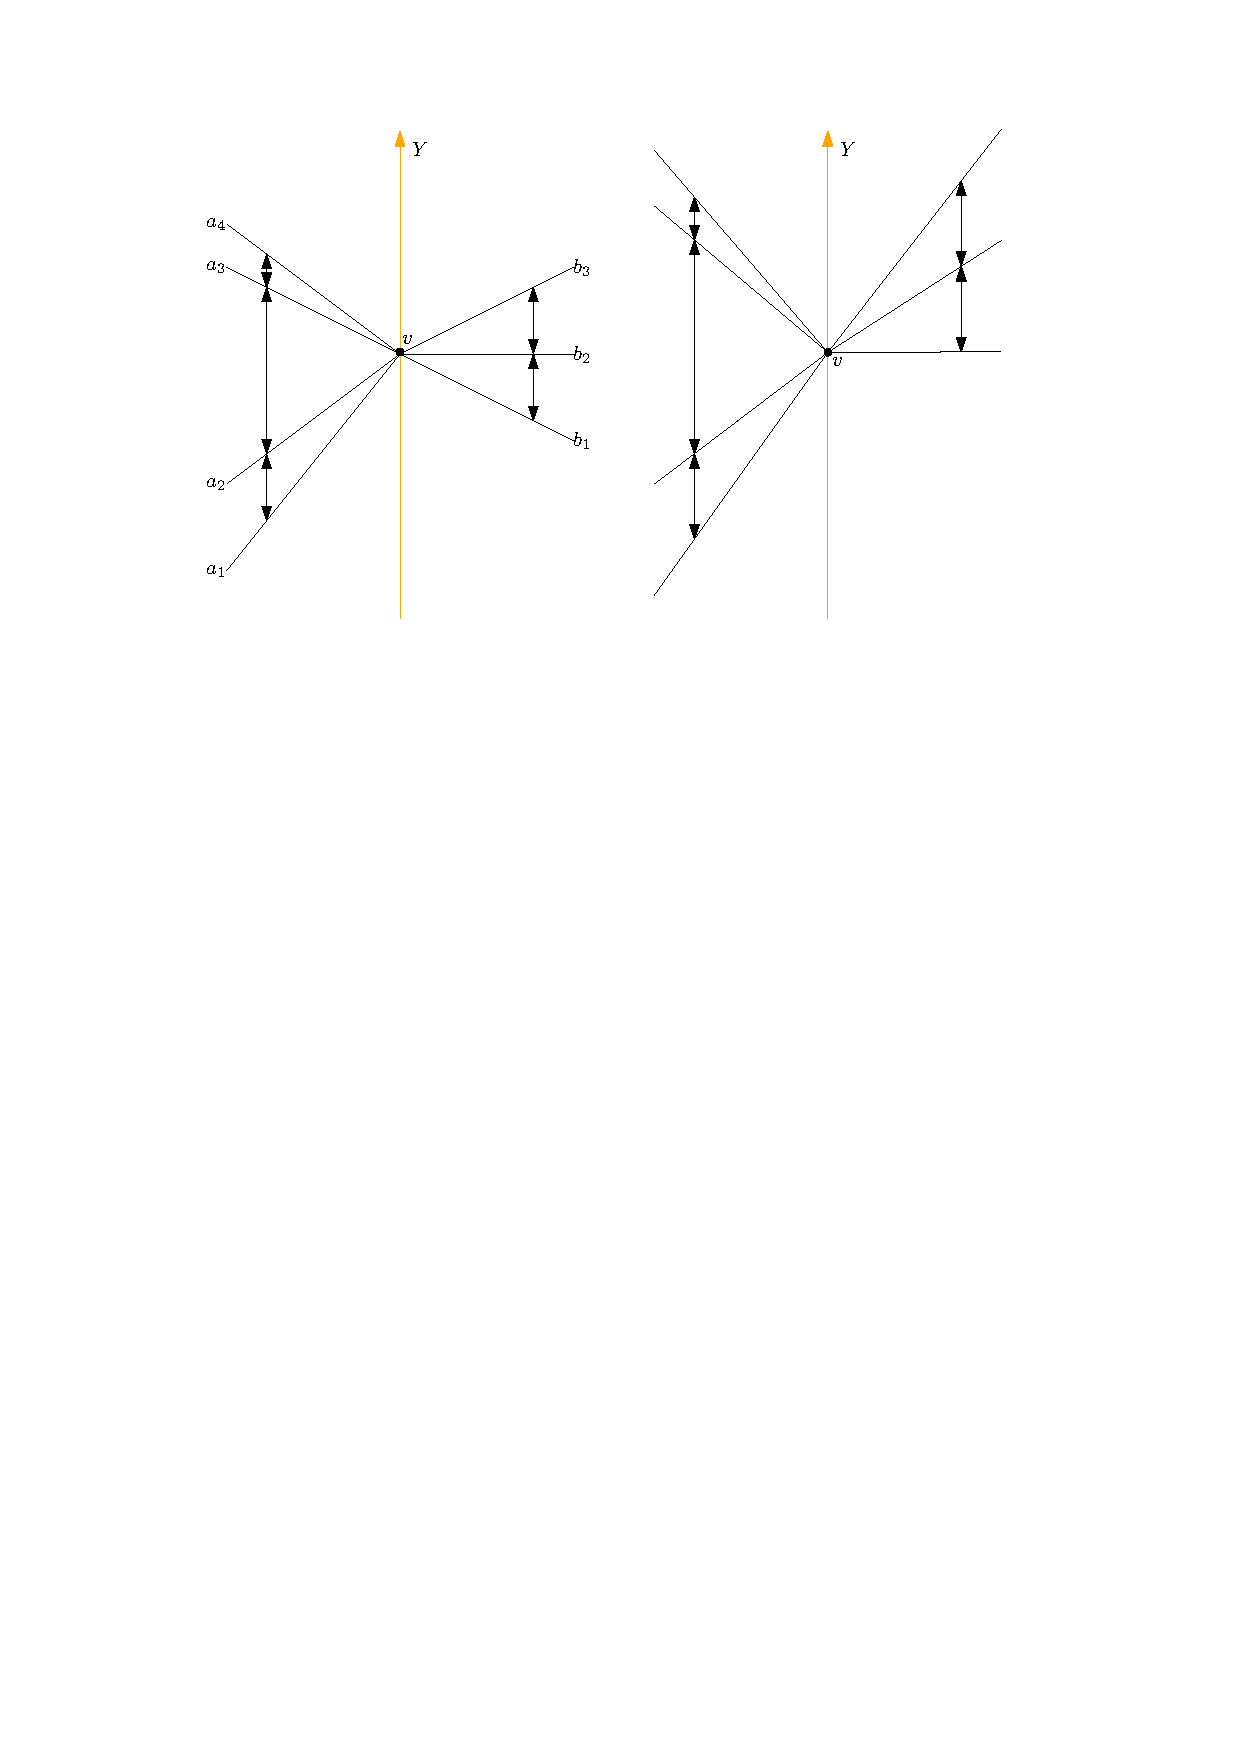
\includegraphics{figs/proportional}}
     \caption{The degrees of freedom provided by the proportionality constraints}
     \figlabel{proportional}
  \end{figure}
The total number of equations
\thetag{\ref{eq:slope0}--\ref{eq:proportion2}} turns out to be $m-4$.
This can be seen as follows: Let $n=|V|$ and let $n_0$ be the number
of vertices on $Y$. Assume that $G$ has $f_3$ triangular and $f_4$
quadrangular faces.

Two triangles for every vertex on $Y$ (Property 5 of A-graphs):
\begin{equation}
  \label{eq:f3}
  f_3 = 2n_0
\end{equation}
Euler's formula:
\begin{equation}
  \label{eq:Euler}
  n + f_3+f_4 = m+2
\end{equation}
Double-counting of edge-face incidences leads to the relation
\begin{equation}
  \label{eq:edge-face}
  3f_3+4f_4=2m.
\end{equation}
We have $d_v-3$ equations for each of the $n_0$ vertices $v$ on $Y$, if it has
degree $d_v$. For each of the 
 $n-n_0$ vertices $v$ not on $Y$, 
we have $d_v-2$ equations.
  The total number of equations is therefore
  \begin{align*}
 % \label{eq:number-equations2}
P &= 
\sum_{v\in V(G)\cap Y}^n(d_v-3)+
\sum_{v\in V(G)\cap(L\cup R)}^n(d_v-2)
=
\sum_{v\in V}^n(d_v-2)-n_0
=
2m-2n-n_0.
  \end{align*}
Using \thetag{\ref{eq:f3}--\ref{eq:edge-face}}, this can be
simplified to
\begin{align*}
P&=
2m-2n-n_0\\
&= 2m -2n -2f_3-2f_4 +2f_3+2f_4-n_0\\
&= 2m -2(n +f_3+f_4) +\tfrac12(4f_3+4f_4-f_3)\\
&= 2m -2(m+2) +m = m-4.
\end{align*}

To achieve the desired number, $m$, of equations, we have to add
four more equations.  If the outer face is a quadrilateral, we set
the slopes of its 4 edges to fixed values.  If the outer face is a
triangle $\alpha\beta\gamma$, with $\gamma$ on $Y$, we set the slopes
of the 3 boundary edges to fixed values. In addition, we pick another
(non-boundary) edge incident to $\gamma$ and set its slope to a fixed
value.  (Together with the proportionality constraints, this effectively
pins all slopes incident to $\gamma$ to fixed values.)

We call these four additional equations the \emph{boundary equations}.
These equations fix the slopes $s_1$, $s_a$, $s_b$, and $s_m$ of four
edges $e_1$, $e_a$, $e_b$, and $e_m$.

Altogether, we have now a system of $m$ linear equations
in the $m$ unknowns $s=(s_1,\ldots,s_m)$, which we can write
compactly as
 $A\cdot s = b$, with a square matrix $A$ whose entries come from
 \thetag{\ref{eq:slope0}--\ref{eq:proportion2}}.
%are the variables we wish to solve for, and $b$ is a column $m$-vector
%whose entries also come from \eqref{slope}.  
Only four entries of
the right-hand side vector
 $b$
are non-zero, due to the four boundary equations.
We will show that $A\cdot s=b$ has a unique
solution and that this solution gives a \Fary\ embedding of $Q$.

\subsubsection{Setting Proportionality Constraints}

Since our plan is to show how to morph the given embedding of $G$ into the desired embedding, it is important that the given embedding satisfy the appropriate system of equations.  
We now specify how the coefficients in the proportionality constraints
are chosen so that they are satisfied by the initial embedding.  The statement of \thmref{a-graph} assumes that $G$ is a
\Fary\ embedding.  In this embedding, every edge $e$ intersects $Y$
in a single point $(0,y_e')$ and has a slope $s_e'$.  For a particular
vertex $v\in Y$, incident to edges $a_1,\ldots,a_k$ and $b_1,\ldots,b_\ell$
as described above, we use the slopes in the given embedding to set the
coefficients in the proportionality constraints.  In the notation used
in \eqref{proportion}, we set
\[
    \lambda_i = (s_{b_i}'-s_{b_1}')/(s_{b_\ell}'-s_{b_1}') 
\]
and in \eqref{proportion2}, we set
\[
    \mu = (s_{a_1}'-s_{a_k}')/(s_{b_\ell}'-s_{b_1}') \enspace .
\]
This ensures that the slopes $s_{e_1}',\ldots,s_{e_m}'$ satisfy the
proportionality constraints.


\subsubsection{Ordering constraints}

Define a relation $\prec$ on line segments where
$e_1 \prec e_2$
if and only if
\begin{enumerate}
  \item $y_{e_1} < y_{e_2}$ and $e_1$ and $e_2$ have a common endpoint $v\in L$; or
  \item $y_{e_1} > y_{e_2}$ and $e_1$ and $e_2$ have a common endpoint $v\in R$.
\end{enumerate}
We say that a vector $s=(s_1,\ldots,s_m)$ \emph{satisfies the ordering
constraints} if $s_{e_1} < s_{e_2}$ for every pair $e_1,e_2\in E(G)$
such that $e_1\prec e_2$.

This definition captures the condition that vertices of $G$ in $L$
(respectively, $R$) should be embedded so that they remain in $L$
(respectively, $R$).  Note that $\prec$ is acyclic since $G$ is an
A-graph and therefore the slopes $s_{e_1}',\ldots,s_{e_m}'$ of edges
in $G$ satisfy the ordering constraints.  This would not be possible if
$\prec$ contained cycles.
%  Indeed, $i_1\prec
% \cdots \prec i_r$ implies that, for each $j\in\{3,\ldots,r\}$, $y_{i_j}\in
% (\min\{y_{i_{j-1}},y_{i_{j-2}}\}, \max\{y_{i_{j-1}},y_{i_{j-2}}\})$. Thus,
% a chain in $\prec$ corresponds to a sequence of strictly nested intervals.

\begin{lem}\lemlabel{order-gives-embedding}
   Any solution $s$ to $A\cdot s=b$ that satisfies
 the ordering constraints % $\prec$
 yields a
   \Fary\ embedding of $G$.
\end{lem}

\begin{proof}
   If $G$ is a plane embedding of a 2-connected graph, then a
   straight-line embedding $G'$ of $G$ is a \Fary\ embedding provided
   that two conditions are met:
(i) For every vertex~$v$, the cyclic order of the
   edges around $v$ in $G'$ is the same as in $G$; and
(ii) every face of $G$ is embedded without crossings in $G'$
(Devillers, Liotta, Preparata, and Tamassia \cite[Lemma~16]{devillers.liotta.ea:checking}).

In our case, $G'$ is a straight-line embedding of $G$ given by a solution
to $A\cdot s = b$ that satisfies the ordering constraints.  


First we show that $G'$ satisfies requirement (i). There are three cases to consider:
\begin{enumerate}
\item $v\not\in Y$. In this case, the slopes of edges incident on $v$
satisfy the ordering constraints by assumption, and hence the order of
incident edges in $G'$ and $G$ agrees.

\item
$v\in Y$, with incident edges $a_1,\ldots,a_k\in
L\cup Y$ and $b_1,\ldots,b_\ell\in Y\cup R$ as in \figref{ab}. 
\begin{enumerate}
\item If
$v$ is a boundary node, then the slopes of $a_1$, $b_1$ and one of
$a_2$ or $b_2$ are fixed by the boundary constraints.  The proportionality
constraints then fix all the slopes of edges incident to $v$ so that
their ordering agrees with that of $G$.

\item If $v$ is an interior vertex then, 
 as discussed above, the proportionality constraints ensure that
the cyclic order of $v$'s incident edges in $G'$ either matches that of $G$, or it is completely reversed, so that the counterclockwise order of vertices around $v$ in $G'$ is $a_1,\ldots,a_k,b_\ell,\ldots,b_1$.
Let us assume for contradiction that the latter case happens:
\begin{equation}
  \label{eq:not-ordered}
s_{b_1}\ge s_{b_\ell}
\text{ and }
s_{a_k}\ge s_{a_1}
\end{equation}
Let $e$ be the third edge of the triangle with edges $a_1$ and $b_1$,
and let 
 $f$ be the third edge of the triangle with edges $a_k$ and $b_\ell$.
Then the ordering constraint for the endpoints of $e$ imply
\begin{math}
  s_{b_1}<s_e<s_{a_1}
\end{math},
and the ordering constraint for the endpoints of $f$ imply
\begin{math}
  s_{a_k}<s_f<s_{b_\ell}
\end{math}.
Together with \eqref{not-ordered}, this leads to a contradiction.
\end{enumerate}
\end{enumerate}

Next we show that $G'$ satisfies requirement (ii). The graph $G$ has two
kinds of faces:
\begin{enumerate}
\item
   If $q=abcd$ is a quadrilateral face in $G$ with no vertex on $Y$,
   then the ordering constraints imply that $q$ is non-crossing in $G'$.
   Otherwise, by Property~3 of A-graphs, $c$ is reflex vertex of $q$ and,
   by Property~5 of A-graphs, $c\not\in Y$.  The vertex $a$ opposite $c$
   is also not in $T$, so so $b\in Y$ and/or $d\in Y$.  In this case,
   the ordering constraints and the proportionality constraints at $b$
   and/or $d$ ensure that $q$ is non-crossing in $G'$.

\item
   For a triangular face $\alpha\beta\gamma$, with $\gamma\in Y$, 
 the ordering constraints on the vertices $\alpha$ and $\beta$
   ensure that the triangle does not degenerate, and is therefore non-crossing, in $G'$.
\end{enumerate}

   Therefore, by the result
of Devillers \etal\
   cited above, $G'$ is a \Fary\ embedding. % of~$Q$.
\end{proof}


\subsubsection{Strong Ordering Constraints}
\label{strong}

For $\epsilon \ge 0$, we say that $s=(s_1,\ldots,s_m)$ satisfies
the \emph{$\epsilon$-strong ordering constraints} if, for each
$i,j\in\{1,\ldots,m\}$ such that $i\prec j$, the inequality
$s_j-s_i > \epsilon$ holds.
% A solution $s$ that satisfies
Clearly, the $\epsilon$-strong
ordering constraints imply the ordering constraints. The following lemma shows
that the converse holds when the equations are satisfied:

\begin{lem}\lemlabel{weak-to-strong}
   Any solution $s$ to $A\cdot s=b$ that satisifies
the ordering constraints
 also satisfies 
   the $\epsilon$-strong ordering constraints
   for all $\epsilon<\min\{|y_i-y_j| : 1\le i< j\le m\}$.
\end{lem}

\begin{proof}
   \lemref{order-gives-embedding} implies that every vertex is
contained in the complement of the outer face of the
   embedding, which in turn is contained in $\Delta\subset[-1,1]^2$.
In particular, every x-coordinate is
in the interval $[-1,1]$.
The vertex incident to $e_i$ and $e_j$ has x-coordinate
   $(y_j-y_i)/(s_j-s_i)$.
From $|(y_j-y_i)/(s_j-s_i)|\le 1$ we derive
   $|s_j-s_i|\ge|y_j-y_i| > \epsilon$.
\end{proof}

\subsubsection{Uniqueness of Solutions Satisfying Ordering Constraints}

The utility of the $\epsilon$-strong ordering constraints is that they
allow us to appeal to continuity. It is impossible 
to violate
the ordering constraints without first violating the
 $\epsilon$-strong ordering constraints.
But since the ordering constraints imply the
 $\epsilon$-strong ordering constraints,
it is not possible
to violate
the ordering constraints at all.
% by showing that, if $A\cdot s=b$
%were to have some undesireable property, then some function which we
%know to be continuous would have a discontinuity.
An example of this argument will be seen in the following proof.

\begin{lem}\lemlabel{unique}
   If $s$ is a solution to $A\cdot s=b$ that satisfies the ordering
   constraints, % $\prec$, 
then $s$ is 
   the unique solution to $A\cdot s=b$.
\end{lem}

\begin{proof}
   Suppose for contradiction that there is a solution $s$ to $A\cdot s=b$ that satisifies the ordering
   constraints, % $\prec$,
   but is not unique.  Since $A\cdot s=b$ is a linear system, there is an entire (at least) 1-parameter family of solutions,
   i.e., there is a non-zero $m$-vector $r$ such that, for every
   $\lambda\in\mathbb R$, $A(s+\lambda r)=b$.


Define the continuous (in fact, piecewise linear) function
\begin{equation*}
  f(\lambda) := \min \{\, (s_j+\lambda r_j)-(s_i+\lambda r_i) : e_i \prec
  e_j\,\}
,
\end{equation*}
and let $\lambda^*$ be the value with the smallest absolute value
 $|\lambda^*|$ such that
 $f(\lambda^*)\le\epsilon/2$.
Such a value $\lambda^*$ exists for the following reason:
   The vector $r=(r_1,\ldots,r_m)$ has at least four zero entries
   $r_1=r_a=r_b=r_m=0$ since the slopes $s_1$, $s_a$, $s_b$, and $s_m$
   are fixed.
  Since $Q$ is connected, this implies
   that there is at least one vertex $v$ with two incident edges $e_k$
   and $e_\ell$ such that $r_k=0$ and $r_\ell\neq 0$. 
   We can thus make $(s_\ell+\lambda r_\ell)-(s_k+\lambda r_k)=0$,
and then $f(\lambda)\le0$.

Now we know that, for $\lambda$ between $0$ and $\lambda^*$,
the differences $s_j-s_i$ for $e_i\prec e_j$ do not change sign.
It follows that the slopes satisfy the ordering constraints throughout
this interval, and
   \lemref{weak-to-strong} implies that $f(\lambda^*)\ge\epsilon$, a contradiction.
%
 % Set $\lambda^* =
 %   (s_i'-s_j')/r_j$ and observe that $s^*=s+\lambda^* r$ is a solution
 %   to $As^*=b$ in which $s_i^*=s_j^*$.  Therefore, $s^*$ is a solution that
 %   does not satisify $\prec$ (the edges $e_i$ and $e_j$
 %   are parallel).  
%
 %   Without loss of generality, assume $\lambda^* >0$. The strict
 %   inequality in the definition of what it means to satisfy $\prec$
 %   implies that the set $\{\lambda\in\mathbb{R}:\text{$s+\lambda
 %   r$ satisfies $\prec$}\}$ is an open set, and this set includes
 %   $0$. Therefore, $\lambda_0=\min\{\lambda \ge 0:\text{$s+\lambda r$
 %   does not satisfy $\prec$}\}$ is well-defined and is greater than 0.
 %   From the discussion above, we know that $\lambda_0\le \lambda^*$.
%
 %   Since $s+\lambda_0 r$ does not satisfy $\prec$, we know that
 %   there is some pair $i,j\in\{1,\ldots,m\}$ such that $i\prec j$
 %   but $s_i+\lambda_0 r_i \ge s_j+\lambda_0 r_j$. Let $f(\lambda)=
 %   s_j+\lambda_0 r_j - s_i+\lambda_0 r_i$, and observe that $f$ is
 %   continuous (in fact, linear) and that $f(\lambda_0)\le 0$.  However,
 %   \lemref{weak-to-strong} implies that $f(\lambda)>\epsilon$ for all
 %   $\lambda <\lambda_0$. This clearly contradicts the continuity of $f$.
 %   We conclude that $s$ must be the unique solution to $A\cdot s=b$.
\end{proof}

The proof of \lemref{unique} was quite explicit (perhaps overly so)
in showing the discontinuity caused by the $\epsilon$-strong ordering
constraints.  In subsequent arguments we will not be quite so explicit.

\subsubsection{A Parametric Family of Linear Systems}

Note that $A$ and $b$ are functions of $y=(y_1,\ldots,y_m)$ and the
four slopes $h=(s_1,s_a,s_b,s_m)$. We make this explicit, by writing
$A_1=A(y,h)$ and $b_1=b(y,h)$.

Let $y'=(y_1',\ldots,y_m')$ and $s'=(s_1',\ldots,s_m')$ denote the
y-intercepts and slopes of the edges in the initial embedding of $G$
and let $h'=(s_1',s_a',s_b's_m')$.
Again, without loss of generality, we assume that every vertex in the initial embedding of $G$ is contained in $[-1,1]^2$.

Consider the system $A(y',h')\cdot s = b(y',h')$.  This system has
at least one solution $s=s'=(s_1',\ldots,s_m')$.  We now define
a continuous family of linear systems that interpolates between the
systems $A(y',h')\cdot s=b(y',h')$ and $A(y,h)\cdot s=b(y,h)$.

For all $0\le t\le 1$ and each $i\in\{1,a,b,m\}$, 
let $s_i(t)=(1-t)s_i' + ts_i$ and let
$h(t)=(s_1(t),s_a(t),s_b(t),s_m(t))$.
Observe that
\[  
    s_a(t)-s_1(t) = (1-t)(s_a'-s_1') + t(s_a-s_1) > 0 \enspace ,
\]
and the same is true for $s_1(t)-s_m(t)$ and $s_m(t)-s_b(t)$.  Let
\[
     \epsilon_1 = \min_{0\le t\le 1}\min\{s_a(t)-s_1(t), s_1(t)-s_m(t), s_m(t)-s_b(t)\}
\]
and observe that $\epsilon_1>0$.

For all $0\le t\le 1$ and each $i\in\{1,\ldots,m\}$, define $y_i(t) = (1-t)y_i' + ty_i$ and define $y(t)=(y_1(t),\ldots,y_m(t))$.
Observe that, for any
$1\le i< j\le m$ and any $0\le t\le 1$,
\[
   y_j(t) - y_i(t) = (1-t)(y'_j-y'_i) + t(y_j-y_i) > 0 \enspace .
\]
Let 
\[    \epsilon_2=\min_{0\le t\le 1}\min\{y_j(t)-y_i(t): 1\le i< j\le m\}
\]
and observe that $\epsilon_2 >0$.  

The entries in $A_t$ and $b_t$ are derived from \eqref{slope0}, and
each entry is a linear function of~$t$.  
%denominators in \eqref{slope} have absolute values bounded from below
%by $\epsilon_2$.  Thus, each entry in $A_t$ and $b_t$ is finite and is a
%uniformly continuous function of $t$.  

Consider the unique quadrilateral $q(t)$ whose edges cross $Y$ at
$y_1(t)$, $y_a(t)$, $y_b(t)$, $y_m(t)$ and have slopes $s_1(t)$,
$s_a(t)$, $s_b(t)$, and $s_m(t)$, respectively.  Note that
$q(t)\subset[-1/\epsilon_1,1/\epsilon_1]\times[-\infty,\infty]$.
Therefore, after scaling x-coordinates by $1/\epsilon_1$,
\lemref{weak-to-strong} applies to $A_t\cdot s =b_t$, so any solution $s$
that satisfies $\prec$ also satisifies the $\epsilon^*$-strong ordering
constraints, for $\epsilon^*=\epsilon_1\cdot\epsilon_2$.

\subsubsection{Existence (and uniqueness) of solutions to $A_t\cdot s=b_t$}


\begin{lem}\lemlabel{uniqueness}
   For every $0\le t\le 1$, the system $A_t\cdot s=b_t$ has a unique solution,
   and this solution satisfies the ordering constraints. % $\prec$.
\end{lem}

\begin{proof}
   Recall that, since $A_t$ is an $m\times m$ matrix, the system $A_t\cdot
   s=b_t$ has a unique solution~$s$ if and only if $\det A_t \neq 0$.
When $\det A_t =0$, the system may have no solutions or
   multiple solutions.  
When $\det A_t\neq 0$, 
   Cramer's Rule states that
the solution
   $s$ is given by $s(t)=(s_1(t),\ldots,s_m(t))$ where, for each
   $i\in\{1,\ldots,m\}$,
   \[ 
       s_i(t) = \frac{\det A_t^i}{\det A_t } \enspace ,
   \]
   and $A_t^i$ denotes the matrix $A_t$ with its $i$th column replaced
   by $b_t$. 
The numerators $\det A_t^i$ and the common
 denominator $\det A_t $ are polynomials in $t$, and therefore
 continuous
functions of $t$.
The solution $s(t)=(s_1(t),\ldots,s_m(t))$ depends continuously on $t$
as long as  $\det A_t\ne0 $.

   We have already established that $A_0\cdot s=b_0$ has a solution $s=s'$
   that satisfies the ordering constraints. Therefore, by \lemref{unique}, this solution
   is unique, so $\det A_0\neq 0$.

Let $t^*$ be the smallest $t>0$
%, if it exists, 
for which 
 $\det A_{t}= 0$. If such a value does not exist we set $t^*=\infty$.
% or $t>1$, we are
% done.

First we argue that for all $t$ in the interval
$0\le t < \min\{1,t^*\}$,
the unique
solution to $A_t\cdot s=b_t$
 satisfies the ordering constraints.
We can establish this by an argument
   similar to the one which shows the uniqueness of $s'$.
Since
 $s(t)$ depends continuously on $t$,
it would first have to violate the  $\epsilon^*$-strong ordering constraints
before violating the ordering constraints, but this contradicts
   \lemref{weak-to-strong}.

Thus, if $t^*>1$, we are done.
Let us therefore assume that $0<t^*\le 1$ and derive a contradiction.
We let $t$ approach $t^*$ from the left, and we ask
whether the limit $s^*=\lim_{t\uparrow t^*}
   s(t)$ exists.
Each function $s_i(t)$ is a quotient of two polynomials.
Thus, for $t\to t^*$ it can either converge to $s_i(t^*)$ in a
continuous way, 
or it diverges to $+\infty$,
or it diverges to $-\infty$.

All solutions $s(t)$ for $t<t^*$ fulfill the equations and
the $\epsilon^*$-strong ordering constraints.
Hence, if the limit exists, by continuity, it also fulfills
the system $A_{t^*}\cdot s^*=b_{t^*}$
and the $\epsilon^*$-strong ordering constraints.
 By \lemref{unique}, the solution $s^*$ is
the unique solution
of $A_{t^*}\cdot s^*=b_{t^*}$, but this contradicts the assumption
$\det A_{t^*}= 0$.

 It remains to rule out the possibility that
 $A_{t^*}\cdot s=b_{t^*}$ has no solutions because
   $\lim_{t\uparrow t^*} s(t)$ does not exist.  Define the set $H=\{e_i\in
   \{e_1,\ldots,e_m\}:\text{$\lim_{t\uparrow t^*} s_i(t)$ exists}\}$.
(The set $H$ corresponds to edges of $G$
   with
   bounded slope; the remaining edges have divergent slopes; they
   become vertical as $t\uparrow t^*$.)
   \begin{prop}\proplabel{set-H}
The set   $H$ has the following
   properties:
%GIVE THESE PROPERTIES A NAME OR PUT THEM IN A LEMMA, SO WE CAN REFER
%TO THEM.
   \begin{compactenum}
    \item $H$ contains the edges
      on the outer face and every edge incident to a vertex of the outer face.
    \item \label{off-C}
If a vertex $v\not\in Y$ has two incident edges in
$H$,
then all $v$'s incident edges belong to $H$.
    \item \label{on-C}
If a vertex $v\in Y$ has two incident edges $vx,vy$ with $x,y\in L$ or $x,y\in R$, then all $v$'s incident edges belong to $H$.
    \item If $e_i \prec e_j \prec e_k$ and $e_i,e_k\in H$, 
      then $e_j\in H$.
   \end{compactenum}
   \end{prop}
Let us see why the set $H$ satisifies Properties 2 and 3.
If $v$ does not lie on $Y$ and two incident edges have a convergent
slope, this means that the location of $v$ is fixed in the limit.
By the concurrency constraints, the slopes of the remaining incident
edges are also determined, by the requirement that the edges go through
the limit location of $v$.

If $v$ lies on $C$, the argument is more elaborate. If $v$ lies on
on the outer face then all incident edges have fixed slopes and are
therefore in $H$.  Let us consider the case that $v$ is an interior
vertex.  As in \figref{ab}, define the incident edges $a_1,\ldots,a_k$
and $b_1,\ldots,b_\ell$.  Let $e$ be the third edge of the triangle with
edges $a_1$ and $b_1$, and let
 $f$ be the third edge of the triangle with edges $a_k$ and $b_\ell$.
Assume without loss of generality that two of the edges $a_i$ on the left
belong to $H$. Then, by the proportionality constraints, all left edges
$a_i$ belong to $H$, and moreover, the range $b_\ell-b_1$ of the right
incident edges converges to a bounded limit.  It follows that either
all the right edges $b_j$ converge, or they all diverge to $+\infty$,
or they all diverge to $-\infty$, Then the ordering constraint for the
endpoints of $e$ imply
\begin{math}
  s_{b_1}<s_e<s_{a_1}
\end{math}.
This is inconstent with $\lim s_{b_1}=+\infty$.
The ordering constraint for the endpoints of $f$ imply
\begin{math}
  s_{a_k}<s_f<s_{b_\ell}
\end{math}.
This is inconstent with $\lim s_{b_\ell}=-\infty$.  Thus, the only
possibility is that all incident slopes converge.

Let us now show that $H$ satisifies Property~1.  If $v$ is a boundary
vertex with $v\in Y$ then, as discussed above, all of $v$'s incident edges
have their slopes fixed by the boundary constraints and proportionality
constraints.  If $v\not\in Y$, then the location of $v$ is fixed by the
boundary constraints and therefore the slopes of $v$'s incident edges
are fixed by the requirement that each edge $e_i$ incident to $v$ also
contains $(0,y_i)$.
We have now established that the set $H$ has
 the above four properties.
   \lemref{partition-extended} below shows that such a set
   $H$ contains all edges. All slopes converge, and this 
   completes the proof.
\end{proof}

%Condition 1 in the following lemma is more general that what we need,
%because it allows us to proceed by induction.

The last lemma in this section is proven by induction on something
that begins as an $A$-graph but is then dismantled into something
more general.  A \emph{near-A-graph} is a graph that satisfies all the
conditions of an A-graph except that its outer face can be arbitrarily
complex.  More specifically, each edge of a near-A-graph intersects $Y$
in exactly one point; each inner face is a triangle or quadrilateral;
each triangular face contains one vertex in each of $Y$, $L$, and $R$;
and for every vertex $v$ on $Y$ each of the faces directly above and
below $v$ are either triangular faces or the outer face.

\begin{lem}\lemlabel{partition-extended}
%(TAKES THE ROLE OF PREVIOUS LEMMA 5, now \lemref{partition}.)
  Let $G$ be a a near-A-graph and let $H$
  be a subset of $E(G)$ such that
   \begin{compactenum}
    \item if $v$ is a vertex on the outer face 
      of $G$, then edges incident to $v$ belong to $H$;
    \item
if a vertex $v$ does not lie on $Y$ and has two incident edges in
$H$,
then all its incident edges belong to $H$;
    \item
if a vertex $v$ lies on $Y$ and has two incident edges in
$Y\cup L$ or two incident edges in $Y\cup R$
then all $v$'s incident edges belong to $H$.
    \item if $i \prec j \prec k$ and $i,k\in H$, 
      then $j\in H$.
   \end{compactenum}
   Then $H=E(G)$.
\end{lem}

\begin{proof}
The proof is by induction
   on the lexicographically ordered pair $(f(G),|E(G)|)$, where $f(G)$
is the number of inner faces of $G$. 
More specifically, %In other words
%We prove the claim by dismantling $G$
we will dismantle $G$
 from outside while maintaining
 Conditions 1--4:
\begin{itemize}
\item If $G$ is not 2-connected but has more than one edge, we cut it
  into pieces with fewer edges.
\item If $G$ is 2-connected, we will modify it and reduce it to a
  graph
with fewer interior faces,
keeping the number of edges fixed.
\end{itemize}
Eventually, we reduce to a graph with a single edge, and here the
claim is trivial because the edge belongs to the boundary.

   We refer to the edges of $H$ simply as \emph{$H$-edges}.
% (horizontal edge) if it is
%   in $B$ and a \emph{v-edge} (vertical edge) otherwise.  Thus, we wish
%   to show that all edges of $G$ are h-edges. 
The edges on the outer
   face are called boundary edges.

If $G$ is not connected then we can apply induction to each component
   of $G$ separately. If $G$ has a cut vertex $v$, whose removal
   separates $G$ into components $A_1,\ldots,A_r$ then, for each
   $i\in\{1,\ldots,r\}$, we can apply induction to the subgraph of $G$
   induced by $V(A_i)\cup\{v\}$.  
In these reductions, no new boundary edges appear that were not
previously boundary edges, because each inner face is
a quadrangle or a triangle: $G$ cannot contain a nested (2-connected) component
inside another face.
Some adjacent edges in $G$ might no longer be adjacent
after we cut $G$ into pieces. This can make Conditions 2 and~3 only weaker
when applied to the pieces. Thus, induction is justified.

We are left with the case that $G$ is a 2-connected \emph{near-A-graph}(?) whose outer face 
   is a simple cycle $F$.

Case 1. $F$ contains a vertex $v$ on $C$.
Then we identify an interior triangle $vab$ incident to $v$ and open it up,
merging it into the outer face.
We illustrate the procedure for the case that $ab$ lies below $v$, see
\figref{lemma-y-3}.
Let $u$ and $w$ be the predecessor and successor of $v$ on the
counterclockwise cycle $F$, and assume without loss of generality that $u\in R$.

  \begin{figure}
     \centering{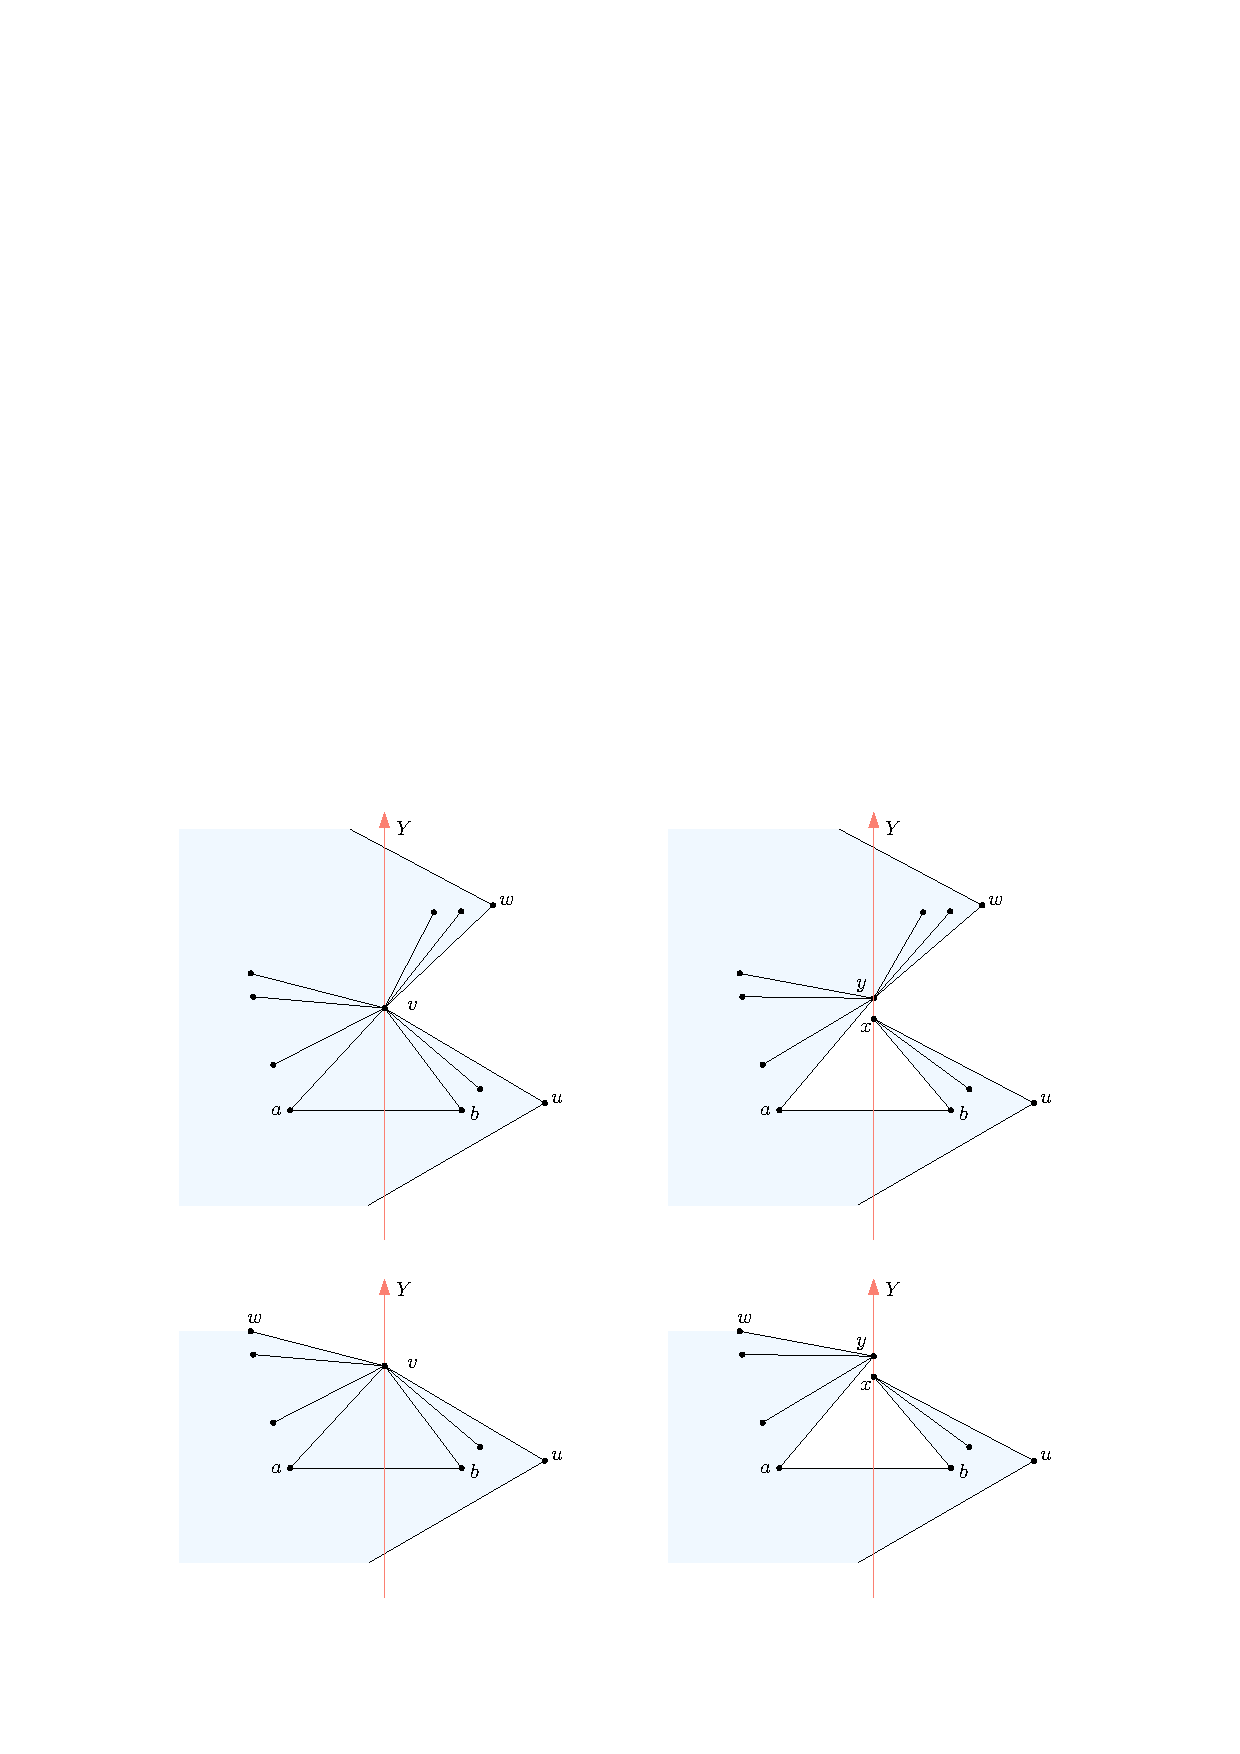
\includegraphics{figs/open-a-triangle}}
     \caption{Proof of \lemref{partition-extended} for a vertex
       $v$ on $C$. Integrating a triangle in the outer face.}
     \figlabel{lemma-y-3}
   \end{figure}


 We construct a new graph $G'$ by splitting $v$ into two vertices $x$
 and $y$ that both lie on $C$, with $y$ above $x$.
 We make $x$ adjacent to $u$ and to every neighbour of
 $v$ between $b$ and $u$.
 We make
 $y$ adjacent to all remaining neighbours of $v$.
\figref{lemma-y-3} shows that this procedure works both for $w\in R$
and for $w\in L$.
 
   In $G'$, the triangle $vab$ has become part of the outer face, so $G'$ has one inner
   face less than $G$, while having the same number of edges.
   
   
Case 2. $F$ contains no vertex on $C$.
Then $F$ contains at least four vertices, and $C$ intersects
   every edge of $F$.  Therefore,  
   $F$
    must contain three consecutive vertices
   $u,v,w$ such that $C$ exits an inner face through $uv$ and enters
   an inner face through $vw$, see \figref{lemma-y-4}.
  This implies that $v$ is a reflex vertex
   of some bounded face $q=vabc$ of $G$.  Indeed, $vc$ is the first edge
   incident to $v$ crossed by $C$ and $va$ is the last such edge.
   %incident to $v$ crossed by $C$.

  \begin{figure}
     \centering{\includegraphics{figs/lemma-y}}
     \caption{Proof of \lemref{partition-extended} for a reflex
       vertex $v$. Integrating a quadrilateral in the outer face.}
     \figlabel{lemma-y-4}
  \end{figure}
   

   We construct a new graph $G'$ by splitting $v$ into two vertices $x$
   and $y$.  We make the vertex $x$ adjacent to $u$ and every neighbour
   $z$ of $v$ such $C$ intersects $vz$ before it intersects $vu$.  We make
   $y$ adjacent to all of $v$'s neighbours that are not adjacent to $x$.
   In $G'$, $q$ is part of the outer face, so $G'$ has one less inner
   face than $G$, while having the same number of edges.

   This finishes the description of how we modify $G$ into $G'$.
Every edge of $G'$ inherits its classification as an $H$-edge from
its corresponding edge in $G$.
   We have
to
show that $G'$ fulfills all assumptions of the lemma.
The only critical assumption is Assumption~1.
All edges incident to the new vertices $x$ or $y$ were incident to $v$
before, and thus they are $H$-edges.

In case of a triangle $vab$, we have two potential new vertices on the
boundary, $a$ and $b$, and they don't lie on~$C$. We know that $va$
and $vb$ are $H$-edges, since they are incident to $v$.
From the ordering constraints around $a$ and $b$ we get
$va\prec ab\prec vb$
or
$vb\prec ab\prec va$, and thus, by Assumption~4, $ab\in H$.
Now we have two $H$-edges $va$ and $vb$ incident to $a$,
and Assumption~2 allows us to conclude that all edges incident
to $a$ belong to $H$, and similarly for~$b$.
   
Let us consider the other case, where we have a quadrilateral 
$q=vabc$.
We have three potential new vertices on the
boundary: $a$, $b$ and $c$. We know that $va$
and $vb$ are $H$-edges, since they are incident to $v$.

As in the triangular case, $va,vc\in H$ by Condition~2.
By looking at the vertices of $q$, we get
$vc \prec bc\prec ba\prec va$ or 
$va \prec ba\prec bc\prec vc$,
 depending on whether $v\in C^-$ or
$v\in C^+$. 
Thus, by Condition~4, $bc$ and $ba$ are also $H$-edges.
The vertex $b$ does not lie on $C$.
The vertex $a$ might lie on $C$ or not, but if it does,
then the two incident edges $va$ and $ab$ lie in the same half-plane.
 The same holds for $d$.
Thus we can apply Assumption~2 or~3, as appropriate,
 to conclude that all edges incident
to $a$, $b$ and $c$ belong to $H$.


   In $G'$ some of the $\prec$-relations involving edges incident
   to $v$ are missing, but no new ones are introduced, so $G'$ still
   satisifies Condition~4.
The same argument applies to
Conditions~2 and~3. Some adjacent edges in $G$ might no longer be adjacent
in $G'$, but this makes Condition 2 and 3 only weaker.

%   By Conditions~1 and 2, all edges incident to $v$ are $H$-edges and $v$
%   is a reflex vertex of $q$. Therefore all edges of $q$ are $H$-edges.
We have justified the induction step for the case when $G$ is
2-connected, and
   the proof is complete.
\end{proof}



%%% Local Variables:
%%% mode: latex
%%% TeX-master: "freecoll"
%%% End:
%XX\subsection{Improper Curves}

\begin{definition}
  An \emph{A-graph} (AD-HOC TERM, THINK OF A BETTER NAME)
is a graph $G$ together with a Jordan curve/arc $C$ that intersects
every edge of $C$ in exactly one point, possibly an endpoint,
and where every vertex on $C$ has at least one incident edge on each side.
\end{definition}

\begin{proposition}
\label  {a-graphs}
A-graphs have the following properties:
\begin{enumerate}
\item Every face, including the outer face, is a quadrilateral or a
  triangle.
\item Every triangle face contains one vertex on $C$, one vertex in
  $L$ and one vertex in $R$.
\item
\label{two-triangles}
  Every $v$ vertex on $C$ is incident to precisely two triangles,
  one 
above $v$ and one below $v$. (This holds also when $v$ is a boundary
vertex; in this case, one of the triangles is the other face.)
\item Every vertex is incident to at least two edges.
\item Every vertex on $C$ is incident to at least three edges.
EXCEPTION: If $v$ is on the outer face, it can have degree 2.
WE MUST EXCLUDE THE DEGREE-2 CASE SOMEWHERE. IT IS TRIVIAL TO HANDLE.
I DON'T KNOW WHERE THE PROPER PLACE FOR HANDLING IT.
\end{enumerate}
\end{proposition}

\begin{thm}\thmlabel{a-graph}
(Generalization of \thmref{quad})

   Let
   \begin{compactenum}
     \item  $G$ be an A-graph;
     \item  $C:[0,1]\to\R^2$ be an admissible Jordan curve for $T$;
     \item $r_1,\ldots,r_k \subseteq E(V)\cup E(G)$ be the sequence of vertices and open edges
           of $T$ that are intersected by $C$, in the order
           that they are intersected by $C$;
     \item $y_1<\cdots<y_k$ be any sequence of numbers; and
     \item .... [$\Delta$ be a triangle that is compatible with 
           $r_1,\ldots,r_m$ and $y_1,\ldots,y_m$.]
  \end{compactenum}
$G$ has a
   \Fary\ embedding in which the outer face $f$ [ is $\Delta$ ]
   and, for each $i\in\{1,\ldots,k\}$, 
   \begin{compactenum}
       \item if $r_i$ is a vertex, then $r_i$ is drawn on the y-axis, with y-coordinate $y_i$;
%       \item if $r_i$ is an edge contained in $C$, then $r_i$ is drawn so that
%         it is contained in the y-axis; or
       \item If $r_i$ is an edge whose intersection with $C$ is a
         single point interior to $r_i$, 
         the intersection of $r_i$ with the
         y-axis has y-coordinate
         $y_i$.
   \end{compactenum}
\end{thm}

\begin{proof}
  We will describe the straight-line embedding by assigning a slope $s_e$
to every edge $e\in E$.
Since there can be no vertical edges, the slopes are well-defined.
We have $m=|E|$ slope variables.

Since every edge goes through a point on the y-axis with known
coordinate, the slope fixes the line through the edge.
 Since
every vertex not on $C$ is incident to at least two edges that go
through
distinct points on the y-axis, location of such a vertex is fixed.

A necessary condition for the slopes is that the lines of edges that
go through a common vertex should be concurrent:
We can extend the function $y$ to all edges, independently of how they
intersect $C$. If $e$ intersects $C$ at an endpoint, we let $y_e$ be
the
given $y$-coordinate of that endpoint. THINK ABOUT A BETTER NOTATION!
%
Let $v$ be a vertex $v$ not on $C$, and let $e_i, e_j, e_k$ be three
edges incident to $v$.
The fact that the three supporting lines of $e_i$, $e_j$, and $e_k$ 
meet at a common point (the location of $v$) is expressed
the following \emph{concurrency constraint} 
in terms of the slopes $s_i,s_j,s_k$:
\begin{equation}\eqlabel{slope0} 
\left|
  \begin{matrix}
    1&1&1\\
s_i&s_j&s_k\\
y_i&y_j&y_k
  \end{matrix}
\right|=
   ({y_j-y_k}) s_i + ({y_k-y_i}) s_j 
          + ({y_i-y_j})s_k  = 0
\end{equation}
Since $y_1,\ldots,y_m$ are given, this is a linear equation
in $s_1,\ldots,s_m$.
Writing this equation for all triplets of edges incident to a common
vertex will include many redundant equations.
If $d_v$ edges meet in a vertex~$v$, 
 It suffices to take $d_v-2$ equations: We choose two fixed
incident edges $e_i$ and $e_j$ and run $e_k$ through the remaining
$d-2$ edges, specifying that $e_k$ should go through the common vertex
of $e_i$ and $e_j$.

It will be important to have as many equations as variables;
thus, we add some more equations for the edges that emanate from a
vertex on $C$.
Suppose that edges $a_1,\ldots,a_k$ 
go to the left and edges $b_1,\ldots,b_l$ go to the
right, from bottom to top.
We have $k,l\ge1$ and $k+l\ge 3$.
Let us first look at the slopes on the right side.
We want these slopes to be increasing:
$s_{b_1} < s_{b_2} < \dots  <s_{b_l}$. We stipulate a stronger
condition:
We require that the slopes
$s_{b_2}, \dots, s_{b_{l-1}}$ partition the interval
$[s_{b_1},s_{b_l}]$ in fixed proportions. In other words
\begin{equation}
  \label{eq:proportion}
s_{b_i} = s_1 + \lambda_i(s_{b_{l}}-s_{b_1}),
\end{equation}
for some fixed sequence $0<\lambda_2<\cdots<\lambda_{l-1}<1$.
For example, we might set $\lambda_i := (i-1)/(l-1)$.
This gives $l-2$ equations, for $l\ge 2$. Similarly, we get
$k-2$ equations for the slopes
$s_{a_1}, \dots, s_{a_{k}}$ on the left side, for $k\ge 2$.
In addition, for $k\ge 2$ and $l\ge 2$, we require that the \emph{range} of
slopes
on the two sides are in a fixed proportion
\begin{equation}
  \label{eq:proportion2}
s_{a_1}-s_{a_{k}} = \mu (s_{b_{l}}-s_{b_1}),
\end{equation}
for some fixed value $\mu>0$.

We call the equations
\thetag{\ref{eq:proportion}--\ref{eq:proportion2}} the
\emph{proportionality constraints}.
There are $(k+l)-3$ such equations for the $k+l$ slopes. In
other words, we have three degrees of freedom for the slopes out of a vertex.
\figref{proportional} illustrates these  degrees of freedom:
We can shear the edges on the right side vertically, adding a constant to all
slopes.
 We can independently shear all edges on the left side.
In addition, we can vertically scale {all} lines jointly (both to
the left and to the right), multiplying all slopes by a constant factor.
If this factor is negative, we would reverse the order of the
slopes. We will later see that other constraints prevent this.
We can already observe that two slopes on one side determine all
remaining slopes on that side. Moreover, the range of slopes
on the other side
($s_{a_1}-s_{a_{k}}$ or $s_{b_{l}}-s_{b_1}$ is also determined.


The notations
$\lambda_i$ and 
$\mu$ are here used in a local sense; for a different vertex $v$, we may
choose different constants.
\begin{figure}
     \centering{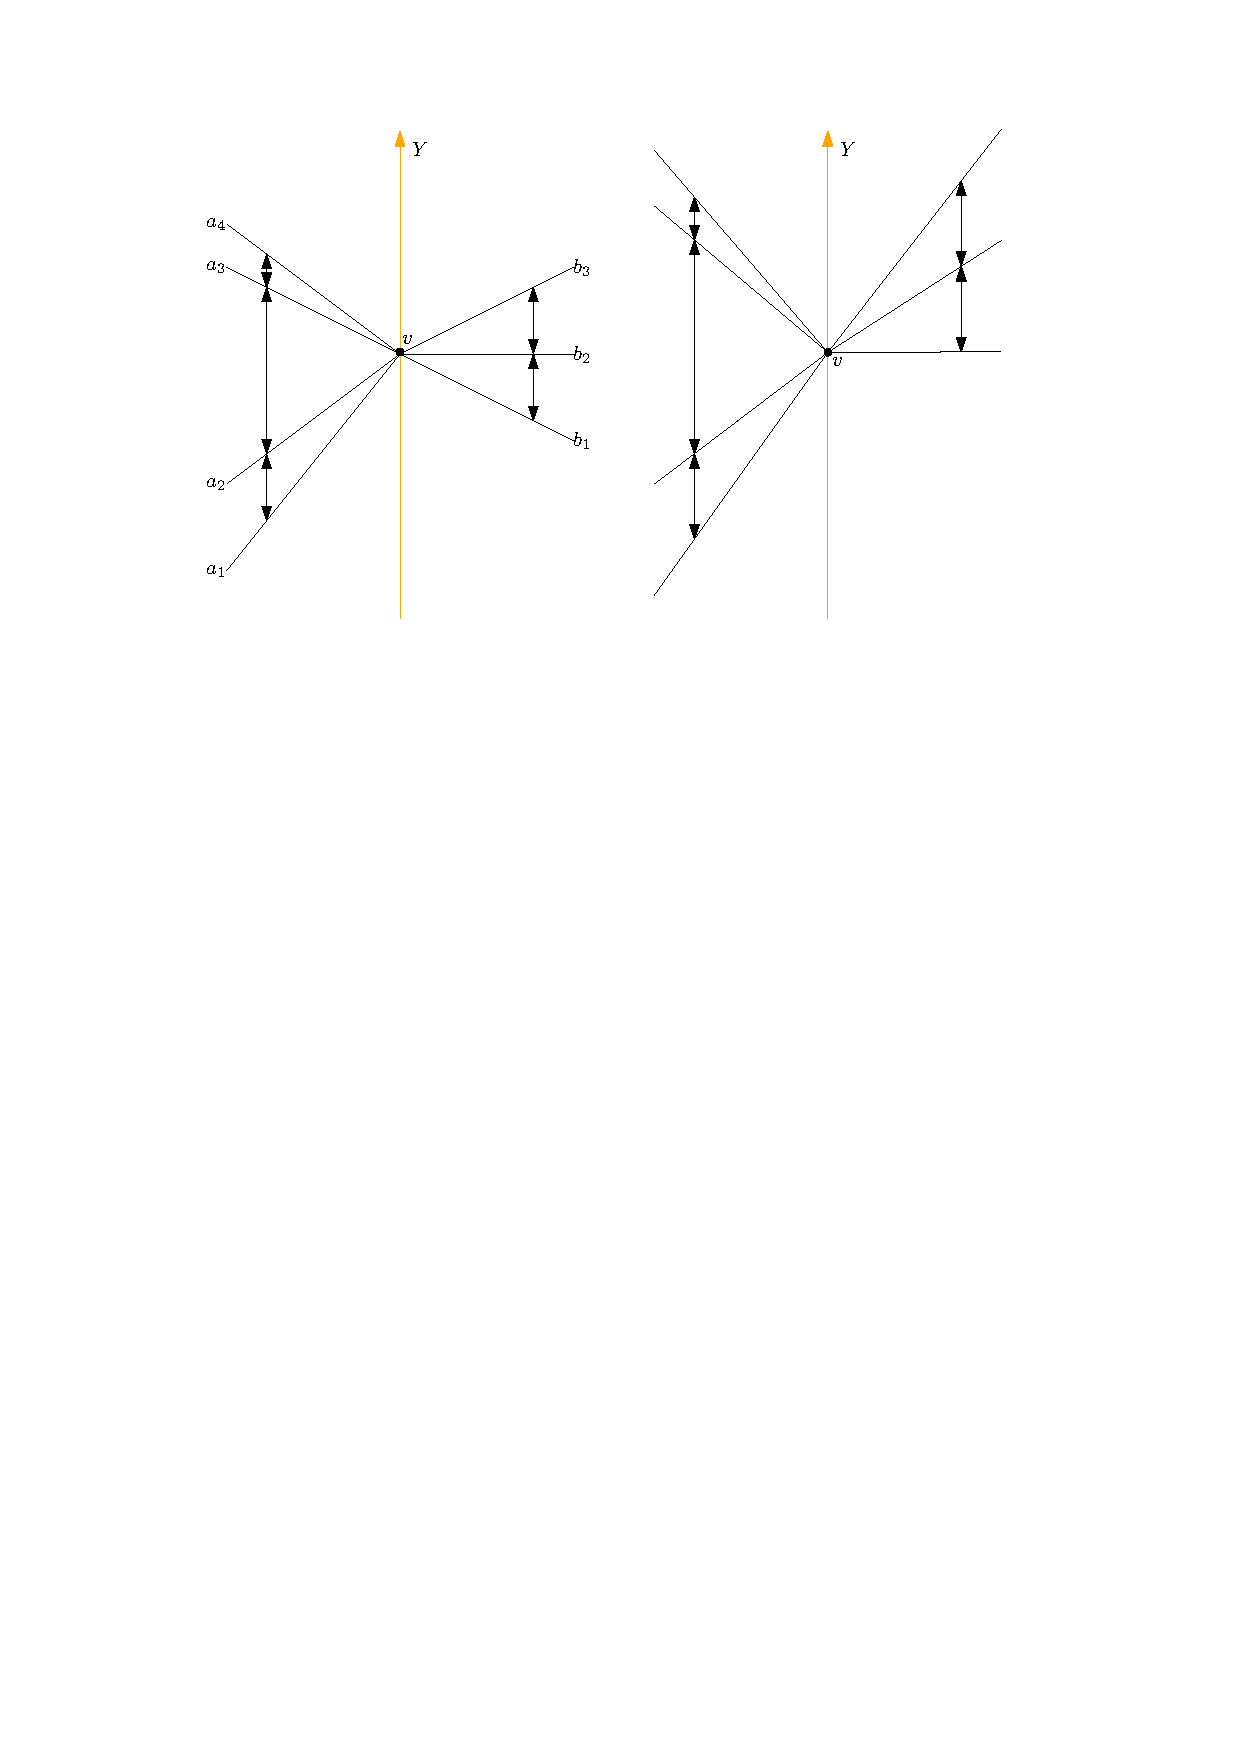
\includegraphics{figs/proportional}}
     \caption{The degrees of freedom provided by the proportionality constraints}
     \figlabel{proportional}
  \end{figure}
The total number of equations
\thetag{\ref{eq:slope0}--\ref{eq:proportion2}} turns out to be $m-4$.
This can be seen as follows: Let $n=|V|$ and let $n_0$ be the number
of vertices on $C$. Assume that $G$ has $f_3$ triangular and $f_4$
quadrangular faces.

Two triangles for every vertex on $C$ (Property \ref{two-triangles}
of Proposition~\ref{a-graphs}):
\begin{equation}
  \label{eq:f3}
  f_3 = 2n_0
\end{equation}
Euler's formula:
\begin{equation}
  \label{eq:Euler}
  n + f_3+f_4 = m+2
\end{equation}
Double-counting of edge-face incidences leads to the relation
\begin{equation}
  \label{eq:edge-face}
  3f_3+4f_4=2m.
\end{equation}
We have $d_v-3$ for each of the $n_0$ vertices $v$ on $C$, if it has
degree $d_v$. For each of the 
 $n-n_0$ vertices $v$ not on $C$, 
we have $d_v-2$ equations.
  The total number of equations is therefore
  \begin{align*}
 % \label{eq:number-equations2}
G &= 
\sum_{v\in C}^n(d_v-3)+
\sum_{v\notin C}^n(d_v-2)
=
\sum_{v\in V}^n(d_v-2)-n_0
=
2m-2n-n_0.
  \end{align*}
Using \thetag{\ref{eq:f3}--\ref{eq:edge-face}}, this can be
simplified to
\begin{align*}
G&=
2m-2n-n_0\\
&= 2m -2n -2f_3-2f_4 +2f_3+2f_4-n_0\\
&= 2m -2(n +f_3+f_4) +\tfrac12(4f_3+4f_4-f_3)\\
&= 2m -2(m+2) +m = m-4.
\end{align*}

To achieve the desired number of $m$ equations, we have to add four
more equations.
If the outer face is a quadrilateral, we set the slopes of its
 4 edges
to fixed values.
If the outer face is a triangle $\alpha\beta\gamma$, with $\gamma$ on
$C$, we set the slopes of the 3 boundary edges
to fixed values. In addition, we pick another (non-boundary) edge
incident to $\gamma$ and set its slope to a fixed value.
(Together with the proportionality constraints, this effectively pins
all slopes
incident to $\gamma$ to fixed values.)

We call these four additional equations the \emph{boundary equations}.

Altogether, we have now a system of $m$ linear equations
in the $m$ unknowns $s=(s_1,\ldots,s_m)$, which we can write
compactly as
 $A\cdot s = b$, with a square matrix $A$ whose entries come from
 \thetag{\ref{eq:slope0}--\ref{eq:proportion2}}.
%are the variables we wish to solve for, and $b$ is a column $m$-vector
%whose entries also come from \eqref{slope}.  
Only four entries of
the right-hand side vector
 $b$
are non-zero, due to the four boundary equations.
We will show that $A\cdot s=b$ has a unique
solution and that this solution gives a \Fary\ embedding of $Q$.

\subsubsection{Ordering constraints}

Define a relation $\prec$ on $\{1,\ldots,m\}$ where $i \prec j$
if
\begin{enumerate}
  \item $i < j$ and $e_i$ and $e_j$ are incident to a common vertex
  $v\in C^-$; or
  \item $i > j$ and $e_i$ and $e_j$ are incident to a common vertex $v\in C^+$.
\end{enumerate}
We say that a vector $s=(s_1,\ldots,s_m)$ \emph{satisfies the ordering constraints} if $s_i <
s_j$ for every pair $i,j\in\{1,\ldots,m\}$ such that $i\prec j$.  

This definition captures the condition that vertices inside of $C$
should be drawn to the left of the y-axis and those outside of $C$
should be drawn to the right of the y-axis.  It is straightforward
to verify that $\prec$ is actually a acyclic: We know that a
non-crossing drawing
$\bar D$ with the vertices on the correct side exists, and the slopes
$s_i'$ of that drawing must satisfy the ordering constraints.
%  Indeed, $i_1\prec
% \cdots \prec i_r$ implies that, for each $j\in\{3,\ldots,r\}$, $y_{i_j}\in
% (\min\{y_{i_{j-1}},y_{i_{j-2}}\}, \max\{y_{i_{j-1}},y_{i_{j-2}}\})$. Thus,
% a chain in $\prec$ corresponds to a sequence of strictly nested intervals.

\begin{lem}\lemlabel{order-gives-embedding}
   Any solution $s$ to $A\cdot s=b$ that satisfies
 the ordering constraints % $\prec$
 yields a
   \Fary\ embedding of $Q$.
\end{lem}

\begin{proof}
   If $G$ is a plane embedding of a 2-connected graph, then a
   straight-line embedding $G'$ of $G$ is a \Fary\ embedding provided
   that two conditions are met:
(i) For every vertex~$v$, the cyclic order of the
   edges around $v$ in $G'$ is the same as in $G$; and
(ii) every face of $G$ is embedded without crossings in $G'$
(Devillers, Liotta, Preparata, and Tamassia \cite[Lemma~16]{devillers.liotta.ea:checking}).

In our case, $G=Q$ and $G'=Q'$ is a straight-line embedding $Q'$ of
$Q$ given by a solution to $A\cdot s = b$.  For each vertex $v$ that
does not lie on $C$, the incident slopes satisfy the ordering constraints
by assumption, and hence the order of incident edges in $G'$ and $G$
agrees.

Let us consider a vertex $v$ on $C$, with
incident edges $a_1,\ldots,a_k$ 
on the left and $b_1,\ldots,b_l$ on the
right.
If $v$ is a boundary node, all slopes are fixed, and the cyclic order
is therefore correct.
Let us consider an interior vertex~$v$.
%
 As discussed above, the proportionality constraints ensure that
the cyclic order is either correct, or it is completely reversed on both
sides.
Let us assume for contradiction that the latter case happens:
\begin{equation}
  \label{eq:not-ordered}
s_{b_1}\ge s_{b_l}
\text{ and }
s_{a_k}\ge s_{a_1}
\end{equation}
Let $e$ be the third edge of the triangle with edges $a_1$ and $b_1$,
and let 
 $f$ be the third edge of the triangle with edges $a_k$ and $b_l$.
Then the ordering constraint for the endpoints of $e$ imply
\begin{math}
  s_{b_1}<s_e<s_{a_1}
\end{math},
and the ordering constraint for the endpoints of $f$ imply
\begin{math}
  s_{a_k}<s_f<s_{b_l}
\end{math}.
Together with \eqref{not-ordered}, this leads to a contradiction.

   For every quadrilateral face in $Q'$, the vertices don't lie on
   $C$, and the ordering constraints on the vertices
   ensure that the embedding is non-crossing.
[For a triangular face $\alpha\beta\gamma$, with $\gamma$ on
$C$,
 the ordering constraints on the vertices $\alpha$ and $\beta$
   ensure that the triangle does not degenerate.]
   Therefore, by the result
of Devillers \etal\
   cited above, $Q'$ is a \Fary\ embedding. % of~$Q$.
\end{proof}


\subsubsection{Strong Ordering Constraints}
SAME AS SECTION \ref{strong}

\end{proof}

... UNTIL HERE CAN BE UNCHANGED.

 It remains to rule out the possibility that
 $A_{t^*}\cdot s=b_{t^*}$ has no solutions because
   $\lim_{t\uparrow t^*} s(t)$ does not exist.  Define the set $H=\{e_i\in
   \{e_1,\ldots,e_m\}:\text{$\lim_{t\uparrow t^*} s_i(t)$ exists}\}$.
(The set $H$ corresponds to edges of $Q$
   with
   bounded slope; the remaining edges have divergent slopes; they
   become vertical as $t\uparrow t^*$.)
   \begin{proposition} \label{set-H}
The set   $H$ has the following
   properties:
GIVE THESE PROPERTIES A NAME OR PUT THEM IN A LEMMA, SO WE CAN REFER
TO THEM.
   \begin{enumerate}
    \item $H$ contains the edges
      on the outer face.
    \item \label{off-C}
If a vertex $v$ that does not lie on $C$ has two incident edges in
$H$,
then all its incident edges belong to $H$.
    \item \label{on-C}
If a vertex $v$ that lies on $C$ has two incident edges in
$H$ on the same side of $C$,
then all its incident edges belong to $H$.
    \item If $i \prec j \prec k$ and $e_i,e_k\in H$, 
      then $e_j\in H$.
   \end{enumerate}
   \end{proposition}
Let us see why properties 2 and 3 are true.
If $v$ does not lie on $C$ and two incident edges have a convergent
slope, this means that the location of $v$ is fixed in the limit.
By the concurrency equations, the slopes of the remaining incident
edges are also determined, by the requirement that the edges go through
the limit location of $v$.

If $v$ lies on $C$, the argument is more elaborate. If $v$ lies on
$C$, then all incident edges have fixed slopes and are therefore in
$H$.
Let uus consider the case that $v$ is an interior vertex.
As above, defince the incident edges $a_i$ and $b_j$.
Let $e$ be the third edge of the triangle with edges $a_1$ and $b_1$,
and let 
 $f$ be the third edge of the triangle with edges $a_k$ and $b_l$.
Assume without loss of generality that two of the edges $a_i$ on the
left belong to $H$. Then, by the proportionality constraints, all
left edges $a_i$ belong to $H$, and moreover, the range $b_l-b_1$ of
the right incident edges converges to a bounded limit.
It follows that either all the right edges $b_j$ converge, 
or they all diverge to $+\infty$,
or they all diverge to $-\infty$,
Then the ordering constraint for the endpoints of $e$ imply
\begin{math}
  s_{b_1}<s_e<s_{a_1}
\end{math}.
THERE IS SOME REPETITIVENESS HERE.
This is inconstent with $\lim s_{b_1}=+\infty$.
The ordering constraint for the endpoints of $f$ imply
\begin{math}
  s_{a_k}<s_f<s_{b_l}
\end{math}.
This is inconstent with $\lim s_{b_l}=-\infty$.
Thus, the only possibility is that all incident slopes converge.

We have now established that the set $H$ has
 the above four properties.
   \lemref{partition-extended} below shows that such a set
   $H$ contains all edges. All slopes converge, and this 
   completes the proof.
\qed%\end{proof}

%Condition 1 in the following lemma is more general that what we need,
%because it allows us to proceed by induction.

\begin{lem}\lemlabel{partition-extended}
(TAKES THE ROLE OF PREVIOUS LEMMA 5, now \lemref{partition}.)
  Let $Q$ be a graph (a ``near-A-graph''?) in which every edge is intersected
  by $C$, and each inner face is a triangle or quadrilateral, and each
  vertex on $C$ has neighbors on the left and on the right.  Let $H$
  be a subset of $E(Q)$ such that
   \begin{compactenum}
    \item If $v$ is a vertex on the outer face 
      of $Q$, then all incident edges belong to $H$;
    \item
If a vertex $v$ does not lie on $C$ and has two incident edges in
$H$,
then all its incident edges belong to $H$.
    \item
If a vertex $v$ lies on $C$ and has two incident edges in
$H$ on the same side of $C$,
then all its incident edges belong to $H$.
    \item if $i \prec j \prec k$ and $i,k\in H$, 
      then $j\in H$.
   \end{compactenum}
   Then $H=E(Q)$.
\end{lem}

In order to apply induction,
this lemma applies to a more general class of graphs than we
need,
because if imposes no constraints on the outer face,
and
Assumption 1 is stronger than the corresponding property in
Proposition~\ref{set-H} that we have established above.

%
Let us see why Assumption 1 is true: (DOES THIS ARGUMENT BELONG HERE?)
Initially, a boundary vertex
 can
lie on $C$ as a vertex of a triangle, then all incident edges belong to $H$ because their slopes
are fixed,
or it
 can
lie on $C$ as a reflex vertex of a quadrilateral, then there are two
$H$-edges on the same side,
or it can
lie away from $C$, then again there are two
incident $H$-edges.
In all cases, we can conclude from properties 2 or 3 that all incident edges belong to $H$.


\begin{proof}
The proof is by induction
   on the lexicographically ordered pair $(f(Q),|E(Q)|)$, where $f(Q)$
is the number of inner faces of $Q$. 
More specifically, %In other words
%We prove the claim by dismantling $Q$
we will dismantle $Q$
 from outside while maintaining
 Conditions 1--4:
\begin{itemize}
\item If $Q$ is not 2-connected but has more than one edge, we cut it
  into pieces with fewer edges.
\item If $Q$ is 2-connected, we will modify it and reduce it to a
  graph
with fewer interior faces,
keeping the number of edges fixed.
\end{itemize}
Eventually, we reduce to a graph with a single edge, and here the
claim is trivial because the edge belongs to the boundary.

   We refer to the edges of $H$ simply as \emph{$H$-edges}.
% (horizontal edge) if it is
%   in $B$ and a \emph{v-edge} (vertical edge) otherwise.  Thus, we wish
%   to show that all edges of $Q$ are h-edges. 
The edges on the outer
   face are called boundary edges.

If $Q$ is not connected then we can apply induction to each component
   of $Q$ separately. If $Q$ has a cut vertex $v$, whose removal
   separates $Q$ into components $A_1,\ldots,A_r$ then, for each
   $i\in\{1,\ldots,r\}$, we can apply induction to the subgraph of $Q$
   induced by $V(A_i)\cup\{v\}$.  
In these reductions, no new boundary edges appear that were not
previously boundary edges, because each inner face is
a quadrangle or a triangle: $Q$ cannot contain a nested (2-connected) component
inside another face.
Some adjacent edges in $Q$ might no longer be adjacent
after we cut $Q$ into pieces. This can make Conditions 2 and~3 only weaker
when applied to the pieces. Thus, induction is justified.

We are left with the case that $Q$ is a 2-connected \emph{near-A-graph}(?) whose outer face 
   is a simple cycle $F$.

Case 1. $F$ contains a vertex $v$ on $C$.
Then we identify an interior triangle $vab$ incident to $v$ and open it up,
merging it into the outer face.
We illustrate the procedure for the case that $ab$ lies below $v$, see
\figref{lemma-y-3}.
Let $u$ and $w$ be the predecessor and successor of $v$ on the
counterclockwise cycle $F$, and assume without loss of generality that $u\in R$.

  \begin{figure}
     \centering{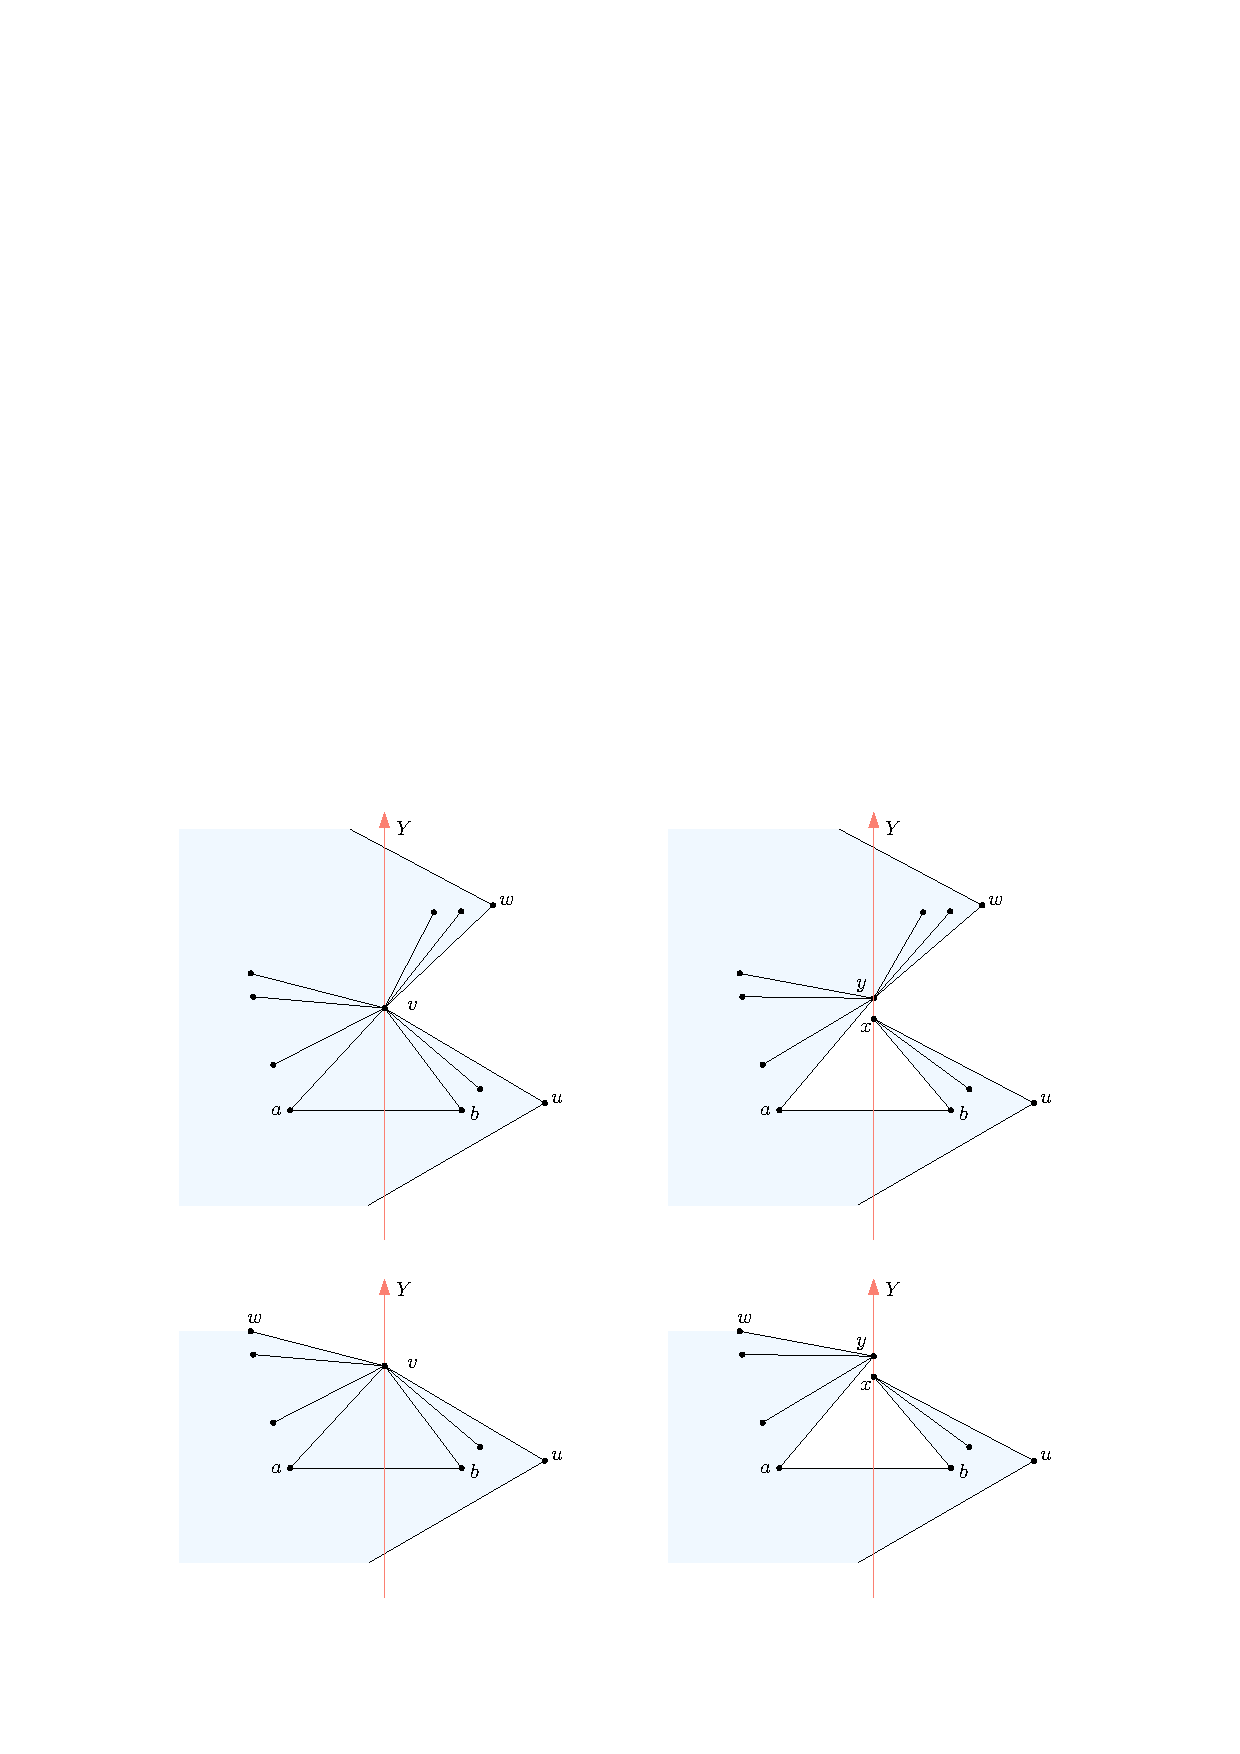
\includegraphics{figs/open-a-triangle}}
     \caption{Proof of \lemref{partition-extended} for a vertex
       $v$ on $C$. Integrating a triangle in the outer face.}
     \figlabel{lemma-y-3}
   \end{figure}


 We construct a new graph $Q'$ by splitting $v$ into two vertices $x$
 and $y$ that both lie on $C$, with $y$ above $x$.
 We make $x$ adjacent to $u$ and to every neighbour of
 $v$ between $b$ and $u$.
 We make
 $y$ adjacent to all remaining neighbours of $v$.
\figref{lemma-y-3} shows that this procedure works both for $w\in R$
and for $w\in L$.
 
   In $Q'$, the triangle $vab$ has become part of the outer face, so $Q'$ has one inner
   face less than $Q$, while having the same number of edges.
   
   
Case 2. $F$ contains no vertex on $C$.
Then $F$ contains at least four vertices, and $C$ intersects
   every edge of $F$.  Therefore,  
   $F$
    must contain three consecutive vertices
   $u,v,w$ such that $C$ exits an inner face through $uv$ and enters
   an inner face through $vw$, see \figref{lemma-y-4}.
  This implies that $v$ is a reflex vertex
   of some bounded face $q=vabc$ of $Q$.  Indeed, $vc$ is the first edge
   incident to $v$ crossed by $C$ and $va$ is the last such edge.
   %incident to $v$ crossed by $C$.

  \begin{figure}
     \centering{\includegraphics{figs/lemma-y}}
     \caption{Proof of \lemref{partition-extended} for a reflex
       vertex $v$. Integrating a quadrilateral in the outer face.}
     \figlabel{lemma-y-4}
  \end{figure}
   

   We construct a new graph $Q'$ by splitting $v$ into two vertices $x$
   and $y$.  We make the vertex $x$ adjacent to $u$ and every neighbour
   $z$ of $v$ such $C$ intersects $vz$ before it intersects $vu$.  We make
   $y$ adjacent to all of $v$'s neighbours that are not adjacent to $x$.
   In $Q'$, $q$ is part of the outer face, so $Q'$ has one less inner
   face than $Q$, while having the same number of edges.

   This finishes the description of how we modify $Q$ into $Q'$.
Every edge of $Q'$ inherits its classification as an $H$-edge from
its corresponding edge in $Q$.
   We have
to
show that $Q'$ fulfills all assumptions.
The only critical assumption is Assumption~1.
All edges incident to the new vertices $x$ or $y$ were incident to $v$
before, and thus they are $H$-edges.

In case of a triangle $vab$, we have two potential new vertices on the
boundary, $a$ and $b$, and they don't lie on~$C$. We know that $va$
and $vb$ are $H$-edges, since they are incident to $v$.
From the ordering constraints around $a$ and $b$ we get
$va\prec ab\prec vb$
or
$vb\prec ab\prec va$, and thus, by Assumption~4, $ab\in H$.
Now we have two $H$-edges $va$ and $vb$ incident to $a$,
and Assumption~2 allows us to conclude that all edges incident
to $a$ belong to $H$, and similarly for~$b$.
   
Let us consider the other case, where we have a quadrilateral 
$q=vabc$.
We have three potential new vertices on the
boundary: $a$, $b$ and $c$. We know that $va$
and $vb$ are $H$-edges, since they are incident to $v$.

As in the triangular case, $va,vc\in H$ by Condition~2.
By looking at the vertices of $q$, we get
$vc \prec bc\prec ba\prec va$ or 
$va \prec ba\prec bc\prec vc$,
 depending on whether $v\in C^-$ or
$v\in C^+$. 
Thus, by Condition~4, $bc$ and $ba$ are also $H$-edges.
The vertex $b$ does not lie on $C$.
The vertex $a$ might lie on $C$ or not, but if it does,
then the two incident edges $va$ and $ab$ lie in the same half-plane.
 The same holds for $d$.
Thus we can apply Assumption~2 or~3, as appropriate,
 to conclude that all edges incident
to $a$, $b$ and $c$ belong to $H$.


   In $Q'$ some of the $\prec$-relations involving edges incident
   to $v$ are missing, but no new ones are introduced, so $Q'$ still
   satisifies Condition~4.
The same argument applies to
Conditions~2 and~3. Some adjacent edges in $Q$ might no longer be adjacent
in $Q'$, but this makes Condition 2 and 3 only weaker. (REPETITION!)


%   By Conditions~1 and 2, all edges incident to $v$ are $H$-edges and $v$
%   is a reflex vertex of $q$. Therefore all edges of $q$ are $H$-edges.
We have justified the induction step for the case when $Q$ is
2-connected, and
   the proof is complete.
\end{proof}


END OF NEW STUFF
\hrule


%%% Local Variables:
%%% mode: latex
%%% TeX-master: "freecoll"
%%% End:

%XX
%XX\subsection{Proper Curves}
%XX
%XXThis section is devoted to proving the following result:
%XX
%XX\begin{thm}\thmlabel{quad}
%XX    Let
%XX    \begin{compactitem}
%XX    \item $Q$ be a quadrangulation with outer face $f$; 
%XX    \item $C:[0,1]\to\R^2$ be a proper Jordan curve for $Q$
%XX     that intersects every edge of $Q$;
%XX    \item $e_1,\ldots,e_m$ be the edges of $Q$ in the
%XX    order they are intersected by $C$; 
%XX    \item $y_1<\cdots<y_m$
%XX    be any increasing sequence of numbers; and
%XX    \item $\Delta$ be a triangle that has no vertex on $C$ and intersects the y-axis
%XX     in the segment with endpoints $(0,y_1)$ and $(0,y_m)$.
%XX    \end{compactitem}
%XX    Then $Q$ has a 
%XX\emph{unique}
%XX\Fary\ embedding in which, for each
%XX    $i\in\{1,\ldots,m\}$, the intersection of $e_i$ with the y-axis is
%XX    a single point $(0,y_i)$ and the edges $e_1$ and $e_m$ are mapped
%XX    to the two edges of $\Delta$ that intersect the y-axis.
%XX\end{thm}
%XX
%XXWe will use the notations $Q$, $f$, $C$, $e_1,\ldots,e_m$,
%XX$y_1,\ldots,y_m$, and $\Delta$ that appear in the statement of
%XX\thmref{quad} consistently throughout this section.
%XXWithout loss of generality, we assume that  $\Delta$ %=\alpha\beta\gamma$ 
%XX has two
%XXvertices $\alpha$
%XXand $\beta$
%XX in $L$ and one vertex $\gamma$ in $R$,
%XXand that   $\Delta=\alpha\beta\gamma$ is oriented counterclockwise,
%XXsee \figref{delta}.
%XXI AM USING NOTATIONS L AND R HERE. NEED TO BE INTRODUCED, OR NOTATION ADAPTED.
%XXTHERE IS DUPLICATION WITH LATER DISCUSSION OF DELTA A FEW PARAGRAPHS BELOW.
%XX
%XXThe requirement that the edges $e_1$ and $e_m$ map to $\Delta$
%XXfixes the embedding of the outer face $f$ of $Q$. Indeed, the vertex of
%XX$f$ common to $e_1$ and $e_m$ will be mapped to $\gamma$,
%XXand
%XXthe other two endpoints of $e_1$ and $e_m$ will be mapped
%XXto $\beta$ and $\alpha$, respectively.  The two remaining edges $e_a$
%XXand $e_b$ of $f$
%XXare then fixed by the requirement that they have endpoints at $\alpha$
%XXand $\beta$ and intersect the y-axis in prescribed locations.
%XX
%XX\begin{figure}
%XX   \centering{\includegraphics{figs/delta}}
%XX   \caption{The triangle $\Delta$ fixes the embedding of the outer face of $Q$.}
%XX   \figlabel{delta}
%XX\end{figure}
%XX
%XXIn the remainder of the proof, we will show that the unique embedding
%XXof the outer face $f$ extends uniquely to the rest of the $Q$ so that
%XX the requirements of
%XX\thmref{quad} are fulfilled.  We do this by describing a system of linear equations that
%XXany straight-line embedding that meets the requirements of \thmref{quad}
%XXmust satisfy.  We then show that this system has a unique solution
%XXand that, from this solution, we can extract a \Fary\ embedding of $Q$
%XXthat satisifies the requirements of \thmref{quad}.
%XXThe proof will be somewhat indirect.
%XX%
%XXBy \thmref{dujmovic-frati}, we know that there is some straight-line
%XXdrawing $\bar D$ 
%XXNOTATION FOR DRAWING????
%XX of $Q$
%XXwhose edges intersect $C$ in the right order but not necessarily 
%XXat the right locations.
%XXWe will then morph the drawing in order to move the intersection
%XXto the desired locations.
%XX
%XX
%XX\subsubsection{The Linear System $A\cdot s=b$ of Concurrency Constraints}
%XX
%XXWe model this problem by a system of equations that has $m$ variables
%XX$s_1,\ldots,s_m$ in which $s_i$ is the slope of the edge $e_i$ in the
%XXdesired embedding, so that $e_i$ lies on the line $\{(x,y):y=s_ix
%XX+ y_i\}$.  Note that, since each vertex of $Q$ has degree at least 2,
%XXa straight-line
%XXembedding of $Q$ is completely determined by
%XXthe values of $s_1,\ldots,s_m$.
%XXHowever, the values $s_1,\ldots,s_m$ must fulfill
%XXadditional conditions in order to determine a plane embedding of
%XX$Q$: (i) all edges incident to a common vertex must meet at a common
%XXpoint.
%XX(ii) Moreover, the edges must not cross.
%XX
%XXWithout loss of generality (by reflection through the y-axis and uniform
%XXscaling of all quantities), assume that $\Delta=\alpha\beta\gamma$
%XXhas two vertices $\alpha$ and $\beta$ to the left of the y-axis and
%XXthe third vertex $\gamma$ to the right of the y-axis and is contained
%XXin $[-1,1]^2$.  The outer face, $f$, of $Q$ has four edges $e_1$, $e_a$,
%XX$e_b$, and $e_m$, where $1 < a < b < m$.  As discussed above, the slopes
%XX$s_1$, $s_a$, $s_b$, and $s_m$ are completely determined $\Delta$
%XXtogether with $y_1$, $y_a$,
%XX$y_b$, $y_c$.
%XXConversely, $\Delta$ is determined by
%XX$s_1$, $s_a$, $s_b$, and $s_m$. We will thus forget $\Delta$ and
%XXchoose the nonredundant daty
%XX$y_1,\ldots,y_m$ and
%XX$s_1, s_a, s_b, s_m$
%XXto describe the constraints that we have to fulfill.
%XX
%XXFor a triple of edges $e_i$, $e_j$, and $e_k$ incident to the same
%XXvertex $v$, the three supporting lines of $e_i$, $e_j$, and $e_k$ must
%XXmeet at a common point (the location of $v$). Therefore
%XXthe slopes %, any solution
%XX$s=(s_1,\ldots,s_m)$ must satisfy the following \emph{concurrency constraint}:
%XX\begin{equation}\eqlabel{slope} 
%XX\left|
%XX  \begin{matrix}
%XX    1&1&1\\
%XXs_i&s_j&s_k\\
%XXy_i&y_j&y_k
%XX  \end{matrix}
%XX\right|=
%XX   ({y_j-y_k}) s_i + ({y_k-y_i}) s_j 
%XX          + ({y_i-y_j})s_k  = 0
%XX\end{equation}
%XXSince $y_1,\ldots,y_m$ are given, this is a linear equation
%XXin $s_1,\ldots,s_m$.
%XXWriting this equation for all triplets of edges incident to a common
%XXvertex will include many redundant equations.
%XXIf $d_v$ edges meet in a vertex~$v$, 
%XX It suffices to take $d_v-2$ equations: We choose two fixed
%XXincident edges $e_i$ and $e_j$ and run $e_k$ through the remaining
%XX$d-2$ edges, specifying that $e_k$ should go through the common vertex
%XXof $e_i$ and $e_j$.  The total number of equations is therefore
%XX\begin{equation}
%XX  \label{eq:number-equations}
%XX  \sum_{v=1}^n(d_v-2) = 2m-2n = m-4,
%XX\end{equation}
%XXusing the relation $m=2n-4$ for quadrangulations, which follows from
%XXEuler's formula.
%XX We have four more equations for the specified slopes
%XX$s_1, s_a, s_b, s_m$.
%XX%
%XX% A result of Felsner \etal\ \cite[Lemma~2.7]{felsner.huemer.ea:binary}
%XX% implies that $Q$ has an orientation of its edges so that each vertex
%XX% except those on the outer face has in-degree 2 and each vertex of the
%XX% outer face has in-degree 1.  Let $\vec{Q}$ be the digraph obtained
%XX% from this orientation. We build a $m\times m$ system of equations in
%XX% the following way: For each directed edge $\vec{xy}$ of $\vec{Q}$
%XX% corresponding to the edge $e_i=xy$ in $Q$, we add the constraint
%XX% \eqref{slope} to the system, where $e_j$ and $e_k$ denote the two incoming
%XX% edges of $x$ in $\vec{Q}$ or---if $x$ is on $f$---the two edges of $f$
%XX% that are incident to $x$.
%XX% GR: I DON'T UNDERSTAND THIS CALCULATION. WHERE ARE THE FOUR EXTRA EQUATIONS?
%XX
%XXThis yields a system of $m$ equations
%XXin the $m$ unknowns $s=(s_1,\ldots,s_m)$, which we can write
%XXas
%XX $A\cdot s = b$, with a square matrix $A$ whose entries come from
%XX \eqref{slope}.
%XX%are the variables we wish to solve for, and $b$ is a column $m$-vector
%XX%whose entries also come from \eqref{slope}.  
%XXOnly four entries of
%XXthe right-hand side vector
%XX $b$
%XXare non-zero because the four slopes $s_1$, $s_a$, $s_b$, and $s_m$
%XXare fixed. % by $\Delta$.  
%XXWe will show that $A\cdot s=b$ has a unique
%XXsolution and that this solution gives a \Fary\ embedding of $Q$.
%XX
%XXIt is clear that any solution $s$ to $A\cdot s=b$ determines a
%XXstraight-line embedding of $Q$ that satisfies the conditions of the the
%XXtheorem, but it is not clear that it determines a \Fary\ embedding of $Q$.
%XXIn particular, it could give an embedding in which edges cross each other.
%XXAs a first step, we impose % consider solutions to $A\cdot s=b$ that
%XX                           % satisfy 
%XXsome
%XXordering constraints.
%XX
%XX\subsubsection{Ordering constraints}
%XX
%XXDefine a relation $\prec$ on $\{1,\ldots,m\}$ where $i \prec j$
%XXif
%XX\begin{enumerate}
%XX  \item $i < j$ and $e_i$ and $e_j$ are incident to a common vertex
%XX  $v\in C^-$; or
%XX  \item $i > j$ and $e_i$ and $e_j$ are incident to a common vertex $v\in C^+$.
%XX\end{enumerate}
%XXWe say that a vector $s=(s_1,\ldots,s_m)$ \emph{satisfies the ordering constraints} if $s_i <
%XXs_j$ for every pair $i,j\in\{1,\ldots,m\}$ such that $i\prec j$.  
%XX
%XXThis definition captures the condition that vertices inside of $C$
%XXshould be drawn to the left of the y-axis and those outside of $C$
%XXshould be drawn to the right of the y-axis.  It is straightforward
%XXto verify that $\prec$ is actually a acyclic: We know that a
%XXnon-crossing drawing
%XX$\bar D$ with the vertices on the correct side exists, and the slopes
%XX$s_i'$ of that drawing must satisfy the ordering constraints.
%XX%  Indeed, $i_1\prec
%XX% \cdots \prec i_r$ implies that, for each $j\in\{3,\ldots,r\}$, $y_{i_j}\in
%XX% (\min\{y_{i_{j-1}},y_{i_{j-2}}\}, \max\{y_{i_{j-1}},y_{i_{j-2}}\})$. Thus,
%XX% a chain in $\prec$ corresponds to a sequence of strictly nested intervals.
%XX
%XX\begin{lem}\lemlabel{order-gives-embedding}
%XX   Any solution $s$ to $A\cdot s=b$ that satisfies
%XX the ordering constraints % $\prec$
%XX yields a
%XX   \Fary\ embedding of $Q$.
%XX\end{lem}
%XX
%XX\begin{proof}
%XX   Devillers \etal\ \cite[Lemma~16]{devillers.liotta.ea:checking} show
%XX   that, if $G$ is a plane embedding of a 2-connected graph and $G'$
%XX   is a straight-line embedding of $G$ in which the cyclic order of the
%XX   edges around every vertex in $G'$ is the same as the cyclic order
%XX   of the edges around every vertex in $G$ and every face of $G$
%XX   has a non-crossing embedding in $G'$, then $G'$ is a \Fary\ embedding.
%XX
%XX   In our case, $G=Q$ and $G'=Q'$ is a straight-line embedding $Q'$ of $Q$
%XX   given by a solution to $A\cdot s = b$ that satisifes $\prec$.  Since
%XX   every edge of $Q$ intersects $C$ and the order of $y_1,\ldots,y_m$
%XX   is the same as the order in which $e_1,\ldots,e_m$ intersect $C$, the
%XX   ordering of the edges around each vertex in $Q'$ is the same as in the
%XX   embedding of $Q$. 
%XX
%XX   For every quadrilateral face in $Q'$, the ordering constraints
%XX   ensure that the embedding is non-crossing. Therefore, by the result
%XX   cited above, $Q'$ is a \Fary\ embedding. % of~$Q$.
%XX\end{proof}
%XX
%XX
%XX\subsubsection{Strong Ordering Constraints}
%XX\label{strong}
%XX
%XXFor $\epsilon \ge 0$, we say that $s=(s_1,\ldots,s_m)$ satisfies
%XXthe \emph{$\epsilon$-strong ordering constraints} if, for each
%XX$i,j\in\{1,\ldots,m\}$ such that $i\prec j$, the inequality
%XX$s_j-s_i\ge \epsilon$ holds.
%XX% A solution $s$ that satisfies
%XXClearly, the $\epsilon$-strong
%XXordering constraints imply the ordering constraints. The following lemma shows
%XXthat the converse holds when the equations are satisfied:
%XX
%XX\begin{lem}\lemlabel{weak-to-strong}
%XX   Any solution $s$ to $A\cdot s=b$ that satisifies
%XXthe ordering constraints
%XX also satisfies 
%XX   the $\epsilon$-strong ordering constraints
%XX   for all $\epsilon\le\min\{|y_i-y_j| : 1\le i< j\le m\}$.
%XX\end{lem}
%XX
%XX\begin{proof}
%XX   \lemref{order-gives-embedding} implies that every vertex is
%XXcontained in the outer face of the
%XX   embedding, which in turn is contained in $\Delta\subset[-1,1]^2$.
%XXIn particular, every x-coordinate is
%XXin the interval $[-1,1]$.
%XXThe vertex incident to $e_i$ and $e_j$ has x-coordinate
%XX   $(y_j-y_i)/(s_j-s_i)$.
%XXFrom $|(y_j-y_i)/(s_j-s_i)|\le 1$ we derive
%XX   $|s_j-s_i|\ge|y_j-y_i| \ge \epsilon$.
%XX\end{proof}
%XX
%XX\subsubsection{Uniqueness of solutions satisfying $\prec$}
%XX
%XXThe utility of the $\epsilon$-strong ordering constraints is that they
%XXallow us to appeal to continuity. If is impossible 
%XXto violate
%XXthe ordering constraints without first violating the
%XX $\epsilon$-strong ordering constraints.
%XXBut since the ordering constraints imply the
%XX $\epsilon$-strong ordering constraints,
%XXit is not possible
%XXto violate
%XXthe ordering constraints at all.
%XX% by showing that, if $A\cdot s=b$
%XX%were to have some undesireable property, then some function which we
%XX%know to be continuous would have a discontinuity.
%XXAn example of this argument will be seen in the following proof.
%XX
%XX\begin{lem}\lemlabel{unique}
%XX   If $s$ is a solution to $A\cdot s=b$ that satisfies the ordering
%XX   constraints, % $\prec$, 
%XXthen $s$ is 
%XX   the unique solution to $A\cdot s=b$.
%XX\end{lem}
%XX
%XX\begin{proof}
%XX   Suppose for contradiction that there is a solution $s$ to $A\cdot s=b$ that satisifies the ordering
%XX   constraints, % $\prec$,
%XX   but is not unique.  Since $A\cdot s=b$ is a linear system, there is an entire (at least) 1-parameter family of solutions,
%XX   i.e., there is a non-zero $m$-vector $r$ such that, for every
%XX   $\lambda\in\mathbb R$, $A(s+\lambda r)=b$.
%XX
%XX
%XXDefine the continuous (in fact, piecewise linear) function
%XX\begin{equation*}
%XX  f(\lambda) := \min \{\, (s_j+\lambda r_j)-(s_i+\lambda r_i) : i \prec
%XX  j\,\}
%XX,
%XX\end{equation*}
%XXand let $\lambda^*$ be the value with the smallest absolute value
%XX $|\lambda^*|$ such that
%XX $f(\lambda^*)\le\epsilon/2$.
%XXSuch a value $\lambda^*$ exists for the following reason:
%XX   The vector $r=(r_1,\ldots,r_m)$ has at least four zero entries
%XX   $r_1=r_a=r_b=r_m=0$ since the slopes $s_1$, $s_a$, $s_b$, and $s_m$
%XX   are fixed.
%XX  Since $Q$ is connected, this implies
%XX   that there is at least one vertex $v$ with two incident edges $e_k$
%XX   and $e_\ell$ such that $r_k=0$ and $r_\ell\neq 0$. 
%XX   We can thus make $(s_\ell+\lambda r_\ell)-(s_k+\lambda r_k)=0$,
%XXand then $f(\lambda)\le0$.
%XX
%XXNow we know that, for $\lambda$ between $0$ and $\lambda^*$,
%XXthe differences $s_j-s_i$ for $i\prec j$ do not change sign.
%XXIt follows that the slopes satisfy the ordering constraints throughout
%XXthis interval, and
%XX   \lemref{weak-to-strong} implies that $f(\lambda^*)\ge\epsilon$, a contradiction.
%XX%
%XX % Set $\lambda^* =
%XX %   (s_i'-s_j')/r_j$ and observe that $s^*=s+\lambda^* r$ is a solution
%XX %   to $As^*=b$ in which $s_i^*=s_j^*$.  Therefore, $s^*$ is a solution that
%XX %   does not satisify $\prec$ (the edges $e_i$ and $e_j$
%XX %   are parallel).  
%XX%
%XX %   Without loss of generality, assume $\lambda^* >0$. The strict
%XX %   inequality in the definition of what it means to satisfy $\prec$
%XX %   implies that the set $\{\lambda\in\mathbb{R}:\text{$s+\lambda
%XX %   r$ satisfies $\prec$}\}$ is an open set, and this set includes
%XX %   $0$. Therefore, $\lambda_0=\min\{\lambda \ge 0:\text{$s+\lambda r$
%XX %   does not satisfy $\prec$}\}$ is well-defined and is greater than 0.
%XX %   From the discussion above, we know that $\lambda_0\le \lambda^*$.
%XX%
%XX %   Since $s+\lambda_0 r$ does not satisfy $\prec$, we know that
%XX %   there is some pair $i,j\in\{1,\ldots,m\}$ such that $i\prec j$
%XX %   but $s_i+\lambda_0 r_i \ge s_j+\lambda_0 r_j$. Let $f(\lambda)=
%XX %   s_j+\lambda_0 r_j - s_i+\lambda_0 r_i$, and observe that $f$ is
%XX %   continuous (in fact, linear) and that $f(\lambda_0)\le 0$.  However,
%XX %   \lemref{weak-to-strong} implies that $f(\lambda)>\epsilon$ for all
%XX %   $\lambda <\lambda_0$. This clearly contradicts the continuity of $f$.
%XX %   We conclude that $s$ must be the unique solution to $A\cdot s=b$.
%XX\end{proof}
%XX
%XXThe proof of \lemref{unique} was quite explicit (perhaps overly so)
%XXin showing the discontinuity caused by the $\epsilon$-strong ordering
%XXconstraints.  In subsequent arguments we will not be quite so explicit.
%XX
%XX\subsubsection{A Parametric Family of Linear Systems}
%XX
%XXNote that $A$ and $b$ are functions of $y=(y_1,\ldots,y_m)$ and
%XXthe triangle $\Delta$. As discussed already, $\Delta$, $y_1$, $y_a$,
%XX$y_b$, and $y_m$ uniquely determine the slopes $h=(s_1,s_a,s_b,s_m)$.
%XXWe make this explicit, by writing
%XX$A_1=A(y,h)$ and $b_1=b(y,h)$.
%XX  \thmref{dujmovic-frati}
%XXimplies that there is some straight-line drawing $D'$ of $Q$ and some
%XX$y_1'<\cdots< y_m'$ such that, for each $i\in\{1,\ldots,m\}$, $e_i$
%XXintersects the y-axis in exactly one point $(0,y_i')$.
%XXDUPLICATION WITH ABOVE?
%XX  Again, without
%XXloss of generality, we assume that $\Delta'\subset [-1,1]^2$ and that
%XX$\Delta'$ has two vertices on the left of the y-axis and one vertex on
%XXthe right.
%XX
%XXThus far, we have established that there exists $y'=(y_1',\ldots,y_m')$
%XXand $h'=(s_1',s_a',s_b',s_m')$ such that the system
%XX$A(y',h')\cdot s' = b(y',h')$ has at least one solution
%XX$s'=(s_1',\ldots,s_m')$.  We now define a continuous family of linear
%XXsystems that interpolates between the systems $A(y',h')\cdot
%XXs=b(y',h')$ and $A(y,h)\cdot s=b(y,h)$.
%XX
%XXFor all $0\le t\le 1$ and each $i\in\{1,a,b,m\}$, 
%XXlet $s_i(t)=(1-t)s_i' + ts_i$ and let
%XX$h(t)=(s_1(t),s_a(t),s_b(t),s_m(t))$.
%XXObserve that
%XX\[  
%XX    s_a(t)-s_1(t) = (1-t)(s_a'-s_1') + t(s_a-s_1) > 0 \enspace ,
%XX\]
%XXand the same is true for $s_1(t)-s_m(t)$ and $s_m(t)-s_b(t)$.  Let
%XX\[
%XX     \epsilon_1 = \min_{0\le t\le 1}\min\{s_a(t)-s_1(t), s_1(t)-s_m(t), s_m(t)-s_b(t)\}
%XX\]
%XXand observe that $\epsilon_1>0$.
%XX
%XXFor all $0\le t\le 1$ and each $i\in\{1,\ldots,m\}$, define $y_i(t) = (1-t)y_i' + ty_i$ and define $y(t)=(y_1(t),\ldots,y_m(t))$.
%XXObserve that, for any
%XX$1\le i< j\le m$ and any $0\le t\le 1$,
%XX\[
%XX   y_j(t) - y_i(t) = (1-t)(y'_j-y'_i) + t(y_j-y_i) > 0 \enspace .
%XX\]
%XXLet 
%XX\[    \epsilon_2=\min_{0\le t\le 1}\min\{y_j(t)-y_i(t): 1\le i< j\le m\}
%XX\]
%XXand observe that $\epsilon_2 >0$.  
%XX
%XXThe entries in $A_t$ and $b_t$ are derived from \eqref{slope}, and
%XXeach entry is a linear function of~$t$.  
%XX%denominators in \eqref{slope} have absolute values bounded from below
%XX%by $\epsilon_2$.  Thus, each entry in $A_t$ and $b_t$ is finite and is a
%XX%uniformly continuous function of $t$.  
%XX
%XXConsider the unique quadrilateral $q(t)$ whose edges cross the
%XXy-axis at $y_1(t)$, $y_a(t)$, $y_b(t)$, $y_m(t)$ and have slopes
%XX$s_1(t)$, $s_a(t)$, $s_b(t)$, and $s_m(t)$, respectively.  Note that
%XX$q(t)\subset[-1/\epsilon_1,1/\epsilon_1]\times[-\infty,\infty]$.
%XXTherefore, after scaling x-coordinates by $1/\epsilon_1$,
%XX\lemref{weak-to-strong} applies to $A_t\cdot s =b_t$, so any solution $s$
%XXthat satisfies $\prec$ also satisifies the $\epsilon^*$-strong ordering
%XXconstraints, for $\epsilon^*=\epsilon_1\cdot\epsilon_2$.  
%XX
%XX\subsubsection{Existence (and uniqueness) of solutions to $A_t\cdot s=b_t$}
%XX
%XX
%XX\begin{lem}\lemlabel{uniqueness}
%XX   For every $0\le t\le 1$, the system $A_t\cdot s=b_t$ has a unique solution,
%XX   and this solution satisfies the ordering constraints. % $\prec$.
%XX\end{lem}
%XX
%XX\begin{proof}
%XX   Recall that, since $A_t$ is an $m\times m$ matrix, the system $A_t\cdot
%XX   s=b_t$ has a unique solution~$s$ if and only if $\det A_t \neq 0$.
%XXWhen $\det A_t =0$, the system may have no solutions or
%XX   multiple solutions.  
%XXWhen $\det A_t\neq 0$, 
%XX   Cramer's rule states that
%XXthe solution
%XX   $s$ is given by $s(t)=(s_1(t),\ldots,s_m(t))$ where, for each
%XX   $i\in\{1,\ldots,m\}$,
%XX   \[ 
%XX       s_i(t) = \frac{\det A_t^i}{\det A_t } \enspace ,
%XX   \]
%XX   and $A_t^i$ denotes the matrix $A_t$ with its $i$th column replaced
%XX   by $b_t$. 
%XXThe numerators $\det A_t^i$ and the common
%XX denominator $\det A_t $ are polynomials in $t$, and therefore
%XX continuous
%XXfunctions of $t$.
%XXThe solution $s(t)=(s_1(t),\ldots,s_m(t))$ depends continuously on $t$
%XXas long as  $\det A_t\ne0 $.
%XX
%XX   We have already established that $A_0\cdot s=b_0$ has a solution $s=s'$
%XX   that satisfies the ordering constraints. Therefore, by \lemref{unique}, this solution
%XX   is unique, so $\det A_0\neq 0$.
%XX
%XXLet $t^*$ be the smallest $t>0$
%XX%, if it exists, 
%XXfor which 
%XX $\det A_{t}= 0$. If such a value does not exist we set $t^*=\infty$.
%XX% or $t>1$, we are
%XX% done.
%XX
%XXFirst we argue that for all $t$ in the interval
%XX$0\le t < \min\{1,t^*\}$,
%XXthe unique
%XXsolution to $A_t\cdot s=b_t$
%XX satisfies the ordering constraints.
%XXWe can establish this by an argument
%XX   similar to the one which shows the uniqueness of $s'$.
%XXSince
%XX $s(t)$ depends continuously on $t$,
%XXit would first have to violate the  $\epsilon^*$-strong ordering constraints
%XXbefore violating the ordering constraints, but this contradicts
%XX   \lemref{weak-to-strong}.
%XX
%XXThus, if $t^*>1$, we are done.
%XXLet us therefore assume that $0<t^*\le 1$ and derive a contradiction.
%XXWe let $t$ approach $t^*$ from the left, and we ask
%XXwhether the limit $s^*=\lim_{t\uparrow t^*}
%XX   s(t)$ exists.
%XXEach function $s_i(t)$ is a quotient of two polynomials.
%XXThus, for $t\to t^*$ it can either converge to $s_i(t^*)$ in a
%XXcontinuous way, 
%XXor it diverges to $+\infty$,
%XXor it diverges to $-\infty$.
%XX
%XXAll solutions $s(t)$ for $t<t^*$ fulfill the equations and
%XXthe $\epsilon^*$-strong ordering constraints.
%XXHence, if the limit exists, by continuity, it also fulfills
%XXthe system $A_{t^*}\cdot s^*=b_{t^*}$
%XXand the $\epsilon^*$-strong ordering constraints.
%XX By \lemref{unique}, the solution $s^*$ is
%XXthe unique solution
%XXof $A_{t^*}\cdot s^*=b_{t^*}$, but this contradicts the assumption
%XX$\det A_{t^*}= 0$.
%XX
%XX It remains to rule out the possibility that
%XX $A_{t^*}\cdot s=b_{t^*}$ has no solutions because
%XX   $\lim_{t\uparrow t^*} s(t)$ does not exist.  Define the set $H=\{e_i\in
%XX   \{e_1,\ldots,e_m\}:\text{$\lim_{t\uparrow t^*} s_i(t)$ exists}\}$.
%XX(The set $H$ corresponds to edges of $Q$
%XX   with
%XX   bounded slope; the remaining edges have divergent slopes; they become vertical as $t\uparrow t^*$.)
%XXThe set   $H$ has he following
%XX   properties:
%XX   \begin{enumerate}
%XX    \item $H$ contains the four edges $e_1$, $e_m$, $e_a$ and $e_b$
%XX      on the outer face.
%XX    \item If $e_i,e_k\in H$ and $e_i$ and $e_k$ are incident to a common
%XX      vertex $v$ then $e_j\in H$ for all edges $e_j$ incident to $v$.
%XX    \item If $i \prec j \prec k$ and $e_i,e_k\in H$, 
%XX      then $e_j\in H$.
%XX   \end{enumerate}
%XX   \lemref{partition} below shows that in any such partition, the set
%XX   $H$ contains all edges. All slopes converge, and this 
%XX   completes the proof.
%XX\end{proof}
%XX
%XXCondition 1 in the following lemma is more general that what we need, because it allows us to
%XXproceed by induction.
%XX
%XX\begin{lem}\lemlabel{partition}
%XX   Let $Q$ be a graph in which each inner face is a
%XX   quadrilateral. Let $H$ be a subset of $E(Q)$ such that
%XX   \begin{compactenum}
%XX    \item $H$ contains all edges on the outer face 
%XX      of $Q$;
%XX    \item if $e_i,e_k\in H$ and $e_i$ and $e_k$ are incident to a common
%XX      vertex $v$ then every edge of $Q$ incident to $v$ is in $H$; and
%XX    \item if $i \prec j \prec k$ and $e_i,e_k\in H$, 
%XX      then $e_j\in H$.
%XX   \end{compactenum}
%XX   Then $H=E(Q)$.
%XX\end{lem}
%XX
%XX\begin{proof}
%XXThe proof is by induction
%XX   on the lexicographically-ordered pair $(f(Q),|E(Q)|)$, where $f(Q)$
%XXis the number of inner faces of $Q$. 
%XXMore specifically, %In other words
%XX%We prove the claim by dismantling $Q$
%XXWe will dismantle $Q$
%XX from outside while maintaining
%XX Conditions 1--3:
%XX\begin{itemize}
%XX\item If $Q$ is not 2-connected but has more than one edge, we cut it
%XX  into pieces with fewer edges.
%XX\item If $Q$ is 2-connected, we will modify it and reduce it to a
%XX  graph
%XXwith fewer interior faces,
%XXkeeping the number of edges fixed.
%XX\end{itemize}
%XXEventually, we reduce to a graph with a single edge, and here the
%XXclaim is trivial because the edge belongs to the boundary.
%XX
%XX   We refer to the edges of $H$ simply as \emph{$H$-edges}.
%XX% (horizontal edge) if it is
%XX%   in $B$ and a \emph{v-edge} (vertical edge) otherwise.  Thus, we wish
%XX%   to show that all edges of $Q$ are h-edges. 
%XXThe edges on the outer
%XX   face are called boundary edges.
%XX
%XXIf $Q$ is not connected then we can apply induction to each component
%XX   of $Q$ separately. If $Q$ has a cut vertex $v$, whose removal
%XX   separates $Q$ into components $A_1,\ldots,A_r$ then, for each
%XX   $i\in\{1,\ldots,r\}$, we can apply induction on the subgraph of $Q$
%XX   induced by $V(A_i)\cup\{v\}$.  
%XXIn these reductions, no new boundary edges appear that were not
%XXpreviously boundary edges, because we assumed that each inner face is
%XXa quadrangle: $Q$ cannot contain nested a (2-connected) component
%XXinside another face.
%XXSome adjacent edges in $Q$ might no longer be adjacent
%XXafter we cut $Q$ into pieces. This can make Condition 2 only weaker
%XXwhen applied to the pieces. Thus, induction is justified.
%XX
%XXWe are left with the case that $Q$ is a 2-connected \emph{near-quadrangulation} whose outer face 
%XX   is a simple cycle $F$, see \figref{lemma-y}.
%XX%  The outer face of $Q$ is a  simple cycle,
%XX$F$ contains at least four vertices, and $C$ intersects
%XX   every edge of $F$.  Therefore,  
%XX   $F$
%XX    must contain three consecutive vertices
%XX   $u,v,w$ such that $C$ exits an inner face through $uv$ and enters
%XX   an inner face through $vw$.  This implies that $v$ is a reflex vertex
%XX   of some bounded face $q=vabc$ of $Q$.  Indeed, $vc$ is the first edge
%XX   incident to $v$ crossed by $C$ and $va$ is the last edge incident to
%XX   $v$ crossed by $C$.
%XX
%XX  \begin{figure}
%XX     \centering{\includegraphics{figs/lemma-y}}
%XX     \caption{The proof of \lemref{partition}.}
%XX     \figlabel{lemma-y}
%XX  \end{figure}
%XX   
%XX   We construct a new graph $Q'$ by splitting $u$ into two vertices $x$
%XX   and $y$.  We make the vertex $x$ adjacent to $u$ and every neighbour
%XX   $z$ of $v$ such $C$ intersects $vz$ before it intersects $vu$.  We make
%XX   $y$ adjacent to all of $v$'s neighbours that are not adjacent to $x$.
%XX   In $Q'$, $q$ is part of the outer face, so $Q'$ has one less inner
%XX   face than $Q$, while having the same number of edges.
%XX
%XXWe have to show that the edges of the quadrilateral 
%XX$q=vabc$,
%XXwhich become boundary edges of $Q'$, are $H$-edges.
%XXThe reflex vertex $v$ is incident to two $H$-edges, namely those of
%XX$F$, and therefore, by Condition 2, $va,vc\in H$.
%XXBy looking at the vertices of $q$, we get
%XX$vc \prec bc\prec ba\prec va$ or 
%XX$va \prec ba\prec bc\prec vc$,
%XX depending on whether $v\in C^-$ or
%XX$v\in C^+$. 
%XXThus, by Condition~3, $bc$ and $ba$ are also $H$-edges.
%XX
%XXEvery edge of $Q'$ inherits its classification as an $H$-edge from
%XXits corresponding edge in $Q$.
%XX   In $Q'$ some of the $\prec$ relations involving edges incident
%XX   to $v$ are missing, but no new ones are introduced, so $Q'$ still
%XX   satisifies Condition~3.
%XXThe same argument applies to
%XXCondition~2. Some adjacent edges in $Q$ might no longer be adjacent
%XXin $Q'$, but this makes Condition 2 only weaker. (REPETITION!)
%XX
%XX
%XX   By Conditions~1 and 2, all edges incident to $v$ are $H$-edges and $v$
%XX   is a reflex vertex of $q$. Therefore all edges of $q$ are $H$-edges.
%XXWe have justified the induction step for the case when $Q$ is
%XX2-connected, and
%XX   the proof is complete.
%XX\end{proof}
%XX
%XXThis completes the proof of \thmref{quad}.  We have
%XXactually shown something stronger: for any $y_1'<\cdots<y_m'$ and
%XXany $y_1<\cdots<y_m$, there is a continuous morph
%XXbetween a drawing $Q'$ in which each edge $e_i$ crosses the y-axis at
%XX$y_i'$ and a drawing $Q$ in which each edge $e_i$ crosses the y-axis
%XXat $y_i$.  At any stage in this morph, all edges cross the y-axis and,
%XXfor each edge $e_i$, the crossing point between $e_i$ and the y-axis
%XXmoves linearly from $y_i'$ to $y_i$.
%XX
%XXLet us retrace the essential steps of our proof:
%XX\begin{itemize}
%XX\item Setting up a %n $m\times m$ 
%XXlinear system $As=b$ that, together
%XXwith some constraints on the order of variables, characterizes the
%XXdrawings
%XXthat we want (\lemref{order-gives-embedding}).
%XX\item 
%XXIT LOOKS STRANGE THAT THE ITEM BULLETS ARE LESS INDENTED THAN THE
%XXPARAGRAPHS.
%XX\item A continuity argument, starting from an embedding with
%XX intersection points at arbitrary locations $y_i$, and moving them
%XX to the desired locations.
%XX\item The notion of strong
%XX ordering constraints, which allowed us to conclude
%XX that the ordering constraints cannot become violated if
%XXthe solution $s$ changes continuously
%XX(\lemref{weak-to-strong}).
%XX\end{itemize}
%XXIt was crucial to have a \emph{square} coefficient matrix $A$ in the
%XXfirst step, because this allowed us to
%XXsingle out a unique solition when $\det A\ne0$ and to
%XX exclude the option of having a
%XXunique solution when $\det A=0$.  ...
%XX
%XXBefore moving on, we also note that, for every quadrangulation $Q$, there
%XXexists a proper Jordan curve $C$ for $Q$ that intersects every edge
%XXof $Q$. This follows from the fact that the dual of $Q$ is 4-regular
%XXand therefore Eulerian, along with a standard uncrossing argument.
%XXThis immediately yields the following corollary of \thmref{quad}.
%XX
%XX\begin{cor}
%XX  For every $m$-edge quadrangulation $Q$ and every $y_1<\cdots<y_m$,
%XX  there exits a \Fary\ embedding of $Q$ in which no edge is
%XX  vertical and, for each $i\in\{1,\ldots,m\}$, the embedding has an edge
%XX  that intersects the y-axis at $(0,y_i)$.
%XX\end{cor}
%XX
%XX\subsection{From Quadrangulations to Collinear Sets}
%XX
%XXTo show that a collinear set in a triangulation $T$ is free, we will
%XXreduce $T$ to a graph $Q^*$ that is not quite a quadrangulation.  However,
%XX$Q^*$ can be made into a quadrangulation $Q$ satisfying the requirements
%XXof \thmref{quad} by splitting each vertex on $C$ into a short edge. The
%XXpurpose of this section is to show that, given the drawing of $Q$ from
%XX\thmref{quad}, this splitting can be undone by contracting these split
%XXedges so that each split edge again becomes a vertex that is placed at
%XXthe appropriate place on the y-axis.  We begin with a geometric lemma:
%XX
%XX\begin{lem}\lemlabel{convergence}
%XX  Let $abcd\subset[-1,1]^2$ be a quadrilateral whose edges
%XX  $e_1=ab$, $e_2=bc$, $e_3=cd$ and $e_4=da$ intersect the y-axis at
%XX  $y_1<y_2<y_3<y_4$, and define $\epsilon=y_3-y_2$ and $g=y_4-y_3$.  Then
%XX  the the x-coordinate of $c$ has absolute value at most $\epsilon/g$ and
%XX  the distance between $c$ and $(0,y_2)$ is at most $\sqrt{5}\epsilon/g$.
%XX\end{lem}
%XX
%XX\begin{proof}
%XX  Refer to \figref{convergence}.  Without loss of generality assume
%XX  $a$ and $c$ are the to left of the y-axis and $b$ and $d$ are to
%XX  the right of the y-axis.  Define $r$ and $q$ so that $c=(-r,y_2-q)$
%XX  so that we want to prove $r\le\epsilon/g$ and $\sqrt{r^2+q^2}\le
%XX  \sqrt{5}\epsilon/g$.
%XX
%XX  \begin{figure}
%XX     \centering{\includegraphics{figs/convergence}}
%XX     \caption{The proof of \lemref{convergence}.}
%XX     \figlabel{convergence}
%XX  \end{figure}
%XX
%XX  For each $i\in\{1,\ldots,4\}$, let $s_i$ denote the slope of $e_i$.
%XX  Then $s_2=q/r$, $s_3=(q+\epsilon)/r=s_2+\epsilon/r$.
%XX  The $x$-coordinate of $d$ is
%XX  \begin{align*}
%XX      d_0 & = \frac{g}{s_3-s_4} \\ 
%XX          & > \frac{g}{s_3-s_1} & \text{(since $s_4 > s_1$)} \\
%XX          & > \frac{g}{s_3-s_2} & \text{(since $s_1 > s_2$)}\\
%XX          & = \frac{rg}{\epsilon} \enspace .
%XX  \end{align*}
%XX  But, since $abcd\subset[-1,1]^2$,  $1\ge d_0> rg/\epsilon$.
%XX  Rewriting this gives $r < \epsilon/g$.
%XX
%XX  The $y$-coordinate of $d$ is
%XX  \begin{align*}
%XX     d_1 & = y_4 + d_0 s_4 \\
%XX     & > y_4 + d_0 s_2 & \text{(since $s_4>s_1>s_2$)} \\
%XX     & = y_4 + d_0 \cdot\frac{q}{r} & \text{(since $s_2=q/r$)} \\
%XX     & > y_4 + \frac{rg}{\epsilon}\cdot\frac{q}{r} & \text{(since $d_0>rg/\epsilon$)} \\
%XX     & = y_4 + \frac{gq}{\epsilon} \\
%XX     & > -1 + \frac{gq}{\epsilon} \enspace. \\
%XX  \end{align*}
%XX  Again $1\ge d_1 > -1 + \frac{gq}{\epsilon}$ and rewriting this gives
%XX  $q < 2\epsilon/g$.  Therefore $\sqrt{r^2+q^2} \le \sqrt{5}\epsilon/g$.
%XX\end{proof}
%XX
%XXLet $Q$ be a quadrangulation satisfying the preconditions of
%XX\thmref{quad}. Then we say an edge $xy$ is a \emph{split edge} of $Q$
%XX(with respect to $C$) if the minimal subcurve of $C$ that intersects all
%XXedges of $Q$ incident to $x$ or $y$ does not intersect any other edges
%XXof $Q$. (See \figref{split-edge}.)
%XX
%XX\begin{figure}
%XX   \centering{\includegraphics{figs/split-edge}}
%XX   \caption{A split edge $xy$ in a quadrangulation.  All split edges are shown in bold and the subcurve of $C$ that proves $xy$ is a split edge is highlighted}
%XX   \figlabel{split-edge}
%XX\end{figure}
%XX
%XX\begin{cor}\corlabel{split-edges}
%XX  Let $Q$, $C$, $e_1,\ldots,e_m$, $y_1,\ldots,y_m$, and $\Delta$
%XX  be as in \thmref{quad}.  Let $xy$ be a split edge of $Q$ with
%XX  respect to $C$, let $I=\{i:\text{$e_i$ is incident to $x$ or
%XX  $y$}\}$, let $\epsilon=\max\{|y_i-y_j|:i,j\in I,\, i\neq j\}$, and
%XX  let $g=\min\{|y_i-y_j|: i\in I,\, j\in\{1,\ldots,m\}\setminus I\}$.
%XX  Then, in the drawing of $Q$ produced by \thmref{quad}, the absolute
%XX  value of $x$ and $y$'s x-coordinates is at most $\epsilon/g$ and the
%XX  distance between $x$ and $y$ is at most $2\sqrt{5}\epsilon/g$.
%XX\end{cor}
%XX
%XX\begin{proof}
%XX   The edge $xy$ is incident to two quadrilaterals. Applying
%XX   \lemref{convergence} to one of these establishes the distance bound
%XX   for $x$ and applying \lemref{convergence} to the other establishes
%XX   the distance bound for $y$.
%XX\end{proof}
%XX
%XXA set $S$ of split edges in $Q$ is \emph{independent} if there is no
%XXedge in $Q$ that joins the endpoints of two distinct edges in $S$.
%XXGiven an independent set $S$ of split edges, we define the graph $Q_S$
%XXby contracting each edge $xy$ in $S$ and placing the resulting vertex at
%XXthe intersection of $C$ and $xy$.  Note that, since $S$ is independent,
%XXeach edge of $Q_S$ intersects $C$ in exactly one point (though it may
%XXbe an endpoint).
%XX
%XXWe need a generalization of \thmref{quad} that allows us to prescribe
%XXthe y-coordinates of edges and vertices of $Q_S$ intersected by $C$.
%XXThis results in an annoying case distinction that occurs when $C$ contains
%XXa vertex on the outer face of $Q_S$ (because $S$ contains an edge of the
%XXouter face of $Q$).  To deal with this, we need some restrictions on the
%XXtriangle $\Delta$.  We say that a triangle $\Delta=\alpha\beta\gamma$
%XXis \emph{compatible} with $Q$, $C$, $S$ and $y_1,\ldots,y_m$ if
%XX\begin{compactenum}
%XX  \item $\beta=(0,y_1)$ if $e_1\in S$, otherwise $(0,y_1)$ is in the interior
%XX  of the edge $\beta\gamma$; and
%XX  \item $\alpha=(0,y_m)$ if $e_m\in S$, otherwise $(0,y_m)$ is in the interior
%XX  of the edge $\alpha\gamma$.
%XX\end{compactenum}
%XX
%XX\begin{thm}\thmlabel{quad2}
%XX   Let $Q$, $C$, $e_1,\ldots,e_m$, $y_1,\ldots,y_m$ be as in
%XX  \thmref{quad}, let $S$ be an independent set of split edges in $Q$,
%XX  and let $\Delta$ be a triangle compatible with $Q$, $C$, $S$, and
%XX  $y_1,\ldots,y_m$.  Then $Q$ has a \Fary\ embedding in which, for
%XX  each $i\in\{1,\ldots,m\}$, the intersection of $e_i$ with the y-axis is
%XX  \begin{compactenum}
%XX     \item $(0,y_i)$ if $e_i$ does not share a vertex with any edge in $S$; or
%XX     \item $(0,y_j)$ if $e_i$ shares an endpoint with $e_j\in S$.
%XX  \end{compactenum}
%XX\end{thm}
%XX
%XX\begin{proof}
%XX  This proof is another continuity argument. For any $\epsilon \ge 0$, we define
%XX  $y(\epsilon)=(y_1(\epsilon),\ldots,y_m(\epsilon))$ as follows:
%XX  \begin{enumerate}
%XX    \item $y_i(\epsilon)= y_i$ if $e_i$ is not incident to a split edge.
%XX    \item For each split edge $e_s=xy$, we set $e_s=y_s$.  Assume, without loss of generality, that $x$'s incident edges
%XX  $e_{s+1},\ldots,e_{s+d}$ cross $C$ after $e_s$. Then we
%XX  set $y_{s+\ell}(\epsilon)=y_s+\epsilon\ell/d$, for each
%XX  $\ell\in\{1,\ldots,d\}$.  Similarly, if $y$ has neighbours
%XX  $e_{s-1},\ldots,e_{s-r}$, we set each $y_{s-\ell}(\epsilon)=y_i -
%XX  \epsilon\ell/r$. 
%XX  \end{enumerate}
%XX  In this way, the edges incident to $x$ have $y(\epsilon)$ values evenly
%XX  spaced in the interval $[y_s,y_s+\epsilon]$ and edges incident $y$
%XX  have $y(\epsilon)$ values evently spaced in $[y_s-\epsilon,y_s]$.
%XX
%XX  For all sufficiently small $\epsilon >0$, \thmref{quad} ensures that
%XX  $Q$ has a straight-line drawing $Q_\epsilon$ in which $e_i$ crosses
%XX  the y-axis at $y_i(\epsilon)$. We use $s_i(\epsilon)$ to denote the
%XX  slope of $e_i$ in $Q_\epsilon$.  The drawing $Q_\epsilon$ changes
%XX  continuously with $\epsilon$ so we can ask if $\lim_{\epsilon\downarrow
%XX  0}Q_\epsilon$ exists and, if it does, does it define the straight-line 
%XX  embedding of $Q_S$ that
%XX  we want?  This answer to both questions is yes.  To establish this,
%XX  we first show that there is a $\delta>0$ such that $Q_\epsilon$ satisfies
%XX  the $\delta$-strong ordering constraint for every sufficiently small
%XX  $\epsilon >0$.
%XX
%XX  Let $g=\min\{|y_i-y_j|: i,j\in\{1,\ldots,m\},\, i\neq j\}$ and observe
%XX  that $g>0$ and does not depend on $\epsilon$.  There are two cases
%XX  to consider:
%XX
%XX  \begin{enumerate}
%XX     \item If two edges $e_i$ and $e_j$ are incident to a common
%XX     vertex $x$ that is not the endpoint of an edge in $S$, then
%XX     in $Q_\epsilon$, $e_i$ crosses the y-axis at $y_i(\epsilon) =
%XX     y_i\pm\epsilon$ and $e_j$ crosses at $y_j(\epsilon)=y_j\pm\epsilon$,
%XX     so $|s_i(\epsilon)-s_j(\epsilon)| \ge |y_i-y_j|-2\epsilon \ge
%XX     g-2\epsilon > g/2$ for all $\epsilon < g/4$.
%XX
%XX    \item On the other hand, if $xy=e_s\in S$ and $e_i$ and $e_j$
%XX    are both incident to $x$, then $|y_i(\epsilon)-y_j(\epsilon)|
%XX    \ge \epsilon/\deg(x) > \epsilon/n$.  However, in this case,
%XX    \corref{split-edges} ensures that the x-coordinate of $x$ is at
%XX    most $\epsilon/g$.  But this means that
%XX    \[
%XX       |s_i(\epsilon)-s_j(\epsilon)|(\epsilon/g) 
%XX            \ge |y_i(\epsilon)-y_j(\epsilon)| 
%XX            \ge \epsilon/n \enspace .
%XX    \]
%XX    Rewriting this gives $|s_i(\epsilon)-s_j(\epsilon)| > g/n$.  
%XX  \end{enumerate}
%XX  Therefore, for all $0<\epsilon\le g/4$, $Q_\epsilon$ satisifies the
%XX  $g/n$-strong ordering constraint.
%XX
%XX  At this point, we are done. The same argument used to exclude events
%XX  of Type~3 in the proof of \lemref{uniqueness} shows that, for each
%XX  $i\in\{1,\ldots,m\}$, $\lim_{\epsilon\downarrow 0} s_i(\epsilon)$
%XX  exists, so $s(0)=\lim_{\epsilon\downarrow 0} s(\epsilon)$ exists.
%XX  Furthermore, for all sufficiently small $\epsilon>0$,
%XX  $Q_\epsilon$ satisfies the $\delta$-strong ordering constraints and
%XX  therefore $s(0)$ satisfies the ordering constraints and determines
%XX  a \Fary\ embedding $Q_0$ of $Q_S$ that fulfills the conditions of
%XX  the theorem.
%XX\end{proof}
%XX
%XX
%\footnote{We abuse the term \emph{drawing} here slightly, since we sometimes require that the two endpoints of a clean edge are drawn at the same location.} in which, for each $i\in\{1,\ldots,m\}$, the intersection
%    of $e_i$ with the y-axis is a single point $(0,y_i)$ and the edges
%    $e_1$ and $e_m$ are mapped to the two edges of $\Delta$ that
%    intersect the y-axis.
%\end{lem}
%
%
%\begin{proof}
%   Add artificial constraints on the slopes of edges incident to split edges (and to split edges themselves.
%\end{proof}
%
%

%
%
%
%
%We say that a 
%Next, we present a strengthening of \lemref{quad} that allows vertices
%of $Q$ to be on the curve $C$.  Let $r_1,\ldots,r_m$ be a sequence
%of vertices and edges in a planar graph and let $y_1<\cdots<y_m$ be a
%sequence of numbers.  We say that a triangle $\Delta=\alpha\beta\gamma$
%is \emph{compatible} with $r_1,\ldots,r_m$ and $y_1,\ldots,y_m$ if
%\begin{compactenum}
%  \item $\beta=p_1$ if $r_1$ is a vertex, otherwise $p_1$ in the interior
%  of the edge $\alpha\beta$; and
%  \item $\gamma=p_m$ if $r_m$ is a vertex, otherwise $p_m$ in the interior
%  of the edge $\alpha\gamma$.
%\end{compactenum}
%
%\begin{lem}\lemlabel{quad2}
%    Let
%    \begin{compactitem}
%    \item $Q$ be a quadrangulation with outer face $f$; 
%    \item $C:[0,1]\to\R^2$ be a Jordan curve
%     whose endpoint $C(0)=C(1)$ is in the interior of $f$,
%     whose intersection with each edge of $Q$
%     consists of exactly one point, and for which no vertex of $Q$ on $C$
%     has neighbours both inside and outside of $C$;
%    \item $r_1,\ldots,r_m$ be the edges and vertices of $Q$ in the
%    order they are intersected by $C$; 
%    \item $y_1<\cdots<y_m$
%    be any increasing sequence of numbers; and
%    \item $\Delta$ be a triangle that is compatible with $r_1,\ldots,r_m$ and $y_1,\ldots,y_m$.
%    \end{compactitem}
%    Then $Q$ has a straight-line
%    drawing in which, for each $i\in\{1,\ldots,m\}$, the intersection
%    of $r_i$ with the y-axis is a single point $(0,y_i)$ and three vertices
%    of $f$ are mapped to the vertices of $\Delta$
%\end{lem}
%
%\begin{proof}
%  Add artifical constraints for vertices on $C$.  If, for some reason, that approach fails, then use the argument we worked out for shifting points off of $C$ and then moving them back to the y-axis.
%%   To fix this, first note that any vertex $r_i$ on $C$ is only incident
%   only to crossing edges and therefore the neighbours of $r_i$ are all
%   contained in $R$. Thus, we can deform $C$ in the neighbourhood of $r_i$
%   so that $r_i$ moves into the interior of $L$ and $C$ intersects each
%   of $r_i$'s incident edges $e_1,\ldots,e_d$ in exactly one point.  Now,
%   to apply \lemref{quad} we must specify numbers $y_1',\ldots,y_d'$ where
%   $(0,y_i')$ is the intersection point between $e_j$ and the y-axis.
%   To do this we choose any $y_1'<\cdots<y_d'$ satisfying
%   \[
%       y_{i-1} < y_1' < y_i < y_d' < y_{i+1} \enspace .
%   \]
%   By doing this for each vertex $r_i$ in $C$ we obtain a curve $C'$ and
%   a sequence $y_1''<\cdots<y_m''$ on which we can apply \lemref{quad} to
%   find a drawing of $Q$.  Now this drawing of $Q$ does not yet satisfy
%   the requirements of the theorem because there are vertices $r_i\in
%   C$ that are not in $C'$. However, the choice of $y_1'<\cdots<y_d'$
%   described above ensures that moving the vertex $r_i$ to $(0,y_i)$
%   does not introduce any crossings and gives a drawing of $Q$ that
%   satisfies all the relevant requirements of the theorem.  Finally,
%   in the process of building $Q$ described above, we showed how the
%   drawing of $Q$ can be extended to a drawing of $T$ that satisifies
%   all the requirements of the theorem.
%\end{proof}



%\begin{lem}
%   Let $Q$ be a straight-line drawing of a quadrangulation each of whose edges intersect the
%   y-axis in exactly one point.  Let $v$ be a vertex of $Q$ that is not on
%   the y-axis, whose incident edges $vx_1,\ldots,vx_d$ intersect
%   the y-axis at y-coordinates $y_1'<\cdots<y_d'$, respectively, 
%   and suppose that no
%   other edges of $Q$ intersect the y-axis with y-coordinates in the interval 
%   $[y_1',y_d']$.
%   Then there is a unique index $i\in\{1,\ldots,d\}$ such that
%   \begin{enumerate}
%     \item for every $j\in\{1,\ldots,i-1\}$, all edges incident to $x_j$, aside from $vx_j$ intersect the y-axis below $(0,y_1')$;
%     \item for every $j\in\{i+1,\ldots,d\}$, all edges incident to $x_j$, aside from $vx_j$ intersect the y-axis above $(0,y_d')$; and
%     \item the embedding of $Q$ obtained by moving $v$ to $(0,y_i')$ is a straight-line drawing.
%   \end{enumerate}
%\end{lem}
%
%\begin{proof}
%   For the first two points, suppose on the contrary that there is some
%   pair of indices $k < \ell$ such that $x_k$ is incident to an edge
%   $wx_k$ that crosses the y-axis at some point $p$ above $(0,y_d')$
%   and $x_\ell$ is incident to an edge $ux_\ell$ that crosses the y-axis
%   at some point $q$ below $(0,y_1')$. Consider the triangle $abc$ with
%   $a=(0,y_k')$, $b=x_k$, and $c=p$.  Then the path $v,x_\ell,u$ enters
%   the interior of $abc$ through the segment $ac$ and exits through one of
%   the other two segments.  But this is a contradiction to the assumption
%   that $Q$ is a straight-line drawing, since it implies that one of the
%   edges in this path crosses at least one of the edges $vx_k$ or $wx_k$.
%
%   For the third point, observe 
%\end{proof}

\section{Triangulations}
\seclabel{triangulations}

In this section we prove that every collinear set is free.
We will sometimes make use of this simple fact:
\begin{obs}\obslabel{quad}
  If $q=abcd$ is a simple quadrilateral, then neither of the segments $ac$
  or $bd$ cross any of the edges of $q$.
\end{obs}

As is the case with \thmref{a-graph} there is an annoying case distinction
that occurs when $Y$ contains vertices on the outer face.  Let $T$
be a triangulation and let $r_1,\ldots,r_k$ be sequence of vertices
and edges in $T$, and let $y_1<\cdots<y_k$ be a sequence of numbers.
We say that a triangle $\Delta=\alpha\beta\gamma$ is \emph{compatible}
with $r_1,\ldots,r_m$ and $y_1,\ldots,y_m$ if
\begin{compactenum}
  \item $\beta=(0,y_1)$ if $r_1$ is a vertex, otherwise $(0, y_1)$ in the interior
  of the edge $\beta\gamma$; and
  \item $\alpha=(0,y_m)$ if $r_m$ is a vertex, otherwise $(0,y_m)$ in the interior
  of the edge $\alpha\gamma$.
\end{compactenum}

We are now ready to state our main theorem.

\begin{thm}\thmlabel{main}
   Let
   \begin{compactenum}
     \item $T$ be an admissible triangulation with outer face $f$;
     \item $r_1,\ldots,r_k$ be the sequence of vertices and open edges
           of $T$ that are intersected by $Y$, in the order
           that they are intersected by $Y$;
     \item $y_1<\cdots<y_k$ be any sequence of numbers; and
     \item $\Delta$ be a triangle that is compatible with 
           $r_1,\ldots,r_m$ and $y_1,\ldots,y_m$.
  \end{compactenum}
   Then, for any $\epsilon>0$, $T$ has a
   \Fary\ embedding in which the outer face $f$ is $\Delta$
   and, for each $i\in\{1,\ldots,k\}$, 
   \begin{compactenum}
       \item if $r_i$ is a vertex, then $r_i$ is drawn on the y-axis, with y-coordinate $y_i$;
       \item if $r_i$ is an edge contained in $Y$, then $r_i$ is drawn so that
         it is contained in the y-axis; or
       \item ($r_i$ is an edge whose intersection with $Y$ is a single point) 
         the intersection of $r_i$ with the
         y-axis has a y-coordinate in the interval
         $[y_i-\epsilon,y_i+\epsilon]$.
   \end{compactenum}
\end{thm}

\begin{proof}
%   We call $y_i$ the (desired) \emph{crossing coordinate} for $r_i$. If
%   a \Fary\ embedding contains an edge whose intersection with the
%   y-axis is $\{(0,y)\}$ or a vertex at $(0,y)$, we say that the edge
%   or vertex \emph{crosses the y-axis at $y$}.
%
%   Let $L=C^-$, $R=C^+$.  
   We say that an edge of $T$ is a \emph{marked
   edge} if its intersection with $C$ is non-empty, otherwise it is
   an \emph{unmarked edge}.  A marked edge is a \emph{crossing edge}
   if its intersection with each of $L$ and $R$ is non-empty.  An edge
   that is not a crossing edge is a \emph{non-crossing edge} (and may
   be marked or unmarked). 

%   We prove an extension of the theorem to the case where $T$ is an
%   non-crossing embedded graph whose faces consist of triangles (3-cycles)
%   and quadrilateral (4-cycles) with the resriction that, for every
%   quadrilateral face $q$, all four edges of $q$ are crossing edges.
%   The proof is by induction on the number of non-crossing edges plus the
%   number of vertices of $T$.

%   \paragraph{Base Cases:}
%   There are three base cases tht we handle explicitly.  If $T$ contains
%   2 or fewer crossing edges, If $T$ is the complete graph, $K_4$ on 4
%   vertices, but only has only three crossing edges, then the theorem is
%   also easy to prove directly.  The last base case occurs when all edges
%   of $T$ are crossing edges.  In this case $T$ is bipartite and therefore
%   all its faces are quadrilaterals, so $T$ is a quadrilateralization.
%   This case is handled directly by \lemref{quad2}.
%
%   Thus we may assume that $T$ has at least one non-crossing edge and
%   at least 2 crossing edges.  

   The proof is by induction on $n+t$, where $n$ is the number of
   vertices of $T$ and $t$ is the number of non-crossing edges.
   We begin by describing reductions that allow us to apply the
   inductive hypothesis. When none of these reductions are possible,
   we arrive at our base case. To handle this base case we argue that
   $T$ has a sufficiently simple structure that it can be handled by
   \thmref{a-graph}.  In particular, when no reduction applies, we can
   remove every unmarked edge of $T$ to obtain an A-graph, on which we
   apply \thmref{a-graph}.

   Before continuing, we dispense with one easy special case.  If $Y$
   contains an edge $e$ of the outer face, $f$, then every vertex
   of $G$ is contained in $L\cup Y$ or every vertex of $G$ is contained
   in $Y\cup R$.  In this case, the definition of compatible triangle
   implies that the edge $\alpha\beta$ of $\Delta$ is contained in the
   y-axis.  In this case, we can simply apply Tutte's Convex Embedding
   Theorem to obtain a \Fary\ embedding of $G$ in which $f$ is embedded
   on $\Delta$ with $e$ embedded on $\alpha\beta$, .  This embedding
   satisifies all the conditions of the theorem.  Therefore, for the
   remainder of this proof, we assume that $C$ intersects the interior
   of at least one inner face of $T$.

   \paragraph{Separating Triangles.}
   (See \figref{separating}.)
   If $T$ contains a separating triangle $xyz$ then we remove all vertices
   from the interior of $xyz$ to obtain a graph $T^+$ in which $xyz$
   is a face.  If the interior of $xyz$ does not intersect $C$, then
   we can apply induction on $T^+$ (which has fewer vertices) and then
   use Tutte's Convex Embedding Theorem to draw $T^-$ so that its outer
   faces matches the embedding of $xyz$ in $T^+$.

   Therefore, assume that $xyz$ has a non-empty intersection with $C$.
   Since the intersection of $C$ with each of $xy$, $yz$ and $zx$
   consists of at most a single point, the vertices and edges of $T$
   intersected by $C$ that are not in $T^+$ appear as a contiguous
   subsequence $r_i,\ldots,r_j$.

   \begin{figure}
      \centering{\includegraphics{figs/separating}}
      \caption{Recursing on separating triangles in the proof of
      \thmref{main}}
      \figlabel{separating}
   \end{figure}

   Observe that each of $r_{i-1}$ and $r_{j+1}$ is either an edge
   or vertex of the triangle $xyz$.  Set $\epsilon'$ to be any
   value less than $\min\{\epsilon,y_{i}-y_{i-1}, y_{j+1}-y_j\}$.
   and apply induction on $T^+$ using the value $\epsilon'$
   and the sequences $r_1,\ldots,r_{i-1},r_{j+1},\ldots,r_k$ and
   $y_1,\ldots,y_{i-1},y_{j+1},\ldots,y_k$ to obtain an embedding
   of $T^+$.  In the resulting embedding $xyz$ becomes a triangular face
   $\Delta'$.

   In the resulting embedding, Let $y_{i-1}'$ and $y_{j+1}'$
   be the respective y-coordinates of the intersections of
   $r_{i-1}$ and $r_{j+1}$ with the y-axis.  By our choice of
   $\epsilon'$, $y_{i-1}'<y_i<\cdots<y_j<y_{j+1}'$.  Observe that
   $\Delta'$ is compatible with $r_{i-1},\ldots,r_{j+1}$ and
   $y_{i-1}',y_i,\ldots,y_j,y_{j+1}'$.

   Let $T^-$ be the graph obtained by removing, from $T$, all
   vertices outside of $xyz$.  Now we apply induction on $T^-$ using
   the triangle $\Delta'$ and the sequences $r_{i-1},\ldots,r_{j+1}$ and
   $y_{i-1}',y_i,\ldots,y_{j},y_{j+1}'$.  Combining the embeddings of $T^+$
   and $T^-$ yields an embedding of $T$ that satisfies the requirements of
   the theorem.  Thus, we may assume that $T$ has no separating triangles.

   \paragraph{Contractible Edges:}
   (See \figref{contractible}.)
   We say that a triangular face of $T$ is a \emph{crossing
   face} if it is incident to two crossing edges.  We say that an
   unmarked edge of $T$ is \emph{contractible} if it is not contained
   in the boundary of any crossing face.  
   \begin{figure}
      \centering{\includegraphics{figs/contractible}}
      \caption{Contracting and uncontracting edges in the proof of
      \thmref{main}}
      \figlabel{contractible}
   \end{figure}

   If $T$ contains a contractible edge $xy$ then we contract $xy$ to
   obtain a new vertex $v$ in a smaller triangulation $T'$.   We can then apply
   induction on $T'$ with the value $\epsilon'=\epsilon/2$ to obtain an
   embedding of $T'$ that satisfies all the conditions of the theorem under
   the stronger condition that each crossing edge $e_i$ crosses
   the y-axis in the interval $[y_i-\epsilon/2,y_i+\epsilon/2]$.

   To obtain an embedding of $T$ we uncontract $v$ by placing $x$ and $y$
   within a ball of radius $\epsilon/2$ centered at $v$. (That such
   a placement is always possible is a standard argument.)  Since the
   distance between $y$ and $v$ and the distance between $x$ and $v$ are each at most $\epsilon/2$,
   each crossing edge $r_i$ incident to $x$ or $y$ will cross
   the y-axis in the interval $[y_i-\epsilon,y_i+\epsilon]$, as required.
   Thus we may assume that $T$ has no separating triangles or contractible
   edges.

%   \paragraph{Eraseable edges}
%   We say that a non-crossing edge of $xy$ of $T$ is \emph{eraseable}
%   if neither of its endpoints is on $C$ and both its incident faces
%   intersect $C$.  If $T$ contains an eraseable edge $xy$, then we remove
%   the edge $xy$ from $T$ to obtain smaller graph $T'$ on which we can
%   apply induction. In the resulting drawing of $T'$, $x$ and $y$ lie on
%   a common face (which may be the outer face of $T'$) and are visible.
%   We can therefore add the edge $xy$ to obtain the desired drawing
%   of $T$.

   \paragraph{Flippable edges.}
   (See \figref{flippable}.)
   We say that an unmarked edge $xy$ of $T$ is \emph{flippable} if there
   exists distinct vertices $z$, $a$, $b$, and $c$, such that 
   \begin{compactenum}
      \item $xyb$, $zyc$, $xza$ are crossing faces of $T$;
      \item $xyz$ is a non-crossing face of $T$; and (
      \item $Y$ intersects $za$, $xa$, $xb$, $yb$, $yc$, and $zc$ in this order; or 
      \item or $Y$ intersects $xa$, $xb$, $yb$, $yc$, $zc$, and $za$ in this order).  
   \end{compactenum}
   \begin{figure}
      \centering{\includegraphics{figs/flippable}}
      \caption{Flipping edges in the proof of
      \thmref{main}}
      \figlabel{flippable}
   \end{figure}

   If $T$ contains the flippable edge $xy$ then we remove $xy$ and replace
   it with $zb$ to obtain a new graph $T'$.  Note that, since $T$ has
   no separating triangles, the edge $zb$ is not already present in $T$.
   After choosing a crossing coordinate for $zb$ somewhere between those
   of $xb$ and $yb$ we can then inductively embed $T'$.

   We claim that in the resulting embedding of $T'$, the only open edge
   that intersects the open segment $xy$ is $zb$.  In particular, we must
   ensure that $z$ is not a reflex vertex in the quadrilateral $xbyz$.
   To show this we distinguish between the two possible cases (3 and 4)
   in the definition of flippable edges. In Case~3, The existence of the
   edges $za$ and $zc$ ensure that, in the resulting embedding of $T'$,
   $xcyz$ is convex.  In Case~4, the triangle $zxa$ is convex and $xbyz$
   is contained in this triangle, therefore $z$ is a convex vertex
   of $xbyz$.

   In either case, removing $zb$ from the embedding of $T'$ and replacing
   it with $xy$ yields the desired embedding of $T$.

   \paragraph{Edges in $Y$.}

   If $T$ contains any edge $xy$ that is contained in $Y$, then we treat
   these exactly the same way we treat flippable edges.  In this case,
   $xy$ is incident to two triangles $xyz$ and $yxb$ with $z\in L$ and
   $b\in R$. We remove $xy$ and add $zb$ to obtain a new triangulation
   $T'$ that has one more crossing edge and on which we can apply
   induction.  In the resulting \Fary\ embedding of $T'$, $z$ and $b$ are
   on opposite sides of the y-axis and $x$ and $y$ are on the y-axis, so
   the neither $z$ nor $b$ is a reflex vertex of the quadrilateral $xzyb$.
   Thus, removing $zb$ and adding $xy$ gives a \Fary\ embedding of $T'$.

   \paragraph{The Base Case.}

   Finally, we are left with a situation in which $T$ is a triangulation
   with no separating triangles, no contractible edges, no flippable
   edges, and no edge contained in $C$.  If $T$ is the complete graph
   $K_3$ or $K_4$ on three or four vertices, then the theorem is trivial,
   so we may assume that $T$ has at least 5 vertices.

   Consider an unmarked edge $xy \in L$.  We claim that $xy$ is on the
   boundary of two faces $xyz$ and $yxb$ where $z,b\in\{Y\cup R\}$.
   Since $xy$ is not contractible, at least one of $xyz$ or $yxb$ is a
   crossing triangle, so at least one of $z$ or $b$, say $b$, is in $R$.
   Suppose then, for the sake of contradiction that $z\in L$ and pick up
   a pencil and paper. Since neither $zx$ nor $yz$ is contractible,
   they must be incident to crossing faces $xza$ and $zyc$, respectively.
   If $a=b=c$, then $T$ is the complete graph, $K_4$, on four vertices,
   which we have already ruled out.  Therefore, assume without loss of
   generality that $b\neq c$.  Since $T$ contains no separating triangles,
   we know that $a\neq c$, otherwise $xya$ would separate $z$ from $b$.

   This leaves us in the situation in which we have distinct vertices $x$,
   $y$, $z$, $a$, $b$, $c$, such that $xyz\in L$ and $xyb$, $zyc$, $xza$
   are crossing faces of $T$ and $xyz$ is a non-crossing face of $T$.
   Checking the definition of flippable edge then ensures that at least
   one of $xy$, $yz$, or $zx$ is a flippable edge. This contradicts the
   assumption that $T$ has no flippable edges.

   Symmetrically, every unmarked edge $xy\in R$ is incident to two faces
   $xyz$ and $yxb$ with $z,b\in L\cup Y$.  Note that this implies that
   no face of $T$ contains more then one unmarked edge.

   Thus, every unmarked edge of $T$ is incident to two faces that
   intersect $Y$.  The union of these two faces is a quadrilateral whose
   boundary consists of four edges that intersect $Y$.
   Let $\tilde{G}$
   denote the plane embedded graph obtained by removing all unmarked edges
   from $T$.  By \thmref{dujmovic-frati}, we know that $\tilde G$ has
   a \Fary\ embedding $G$ whose edges and vertices intersect $Y$ in the
   same order as those of $\tilde{G}$.  We claim that $G$ is an A-graph.
   To verify this, we check each of the properties of an A-graph:

   \begin{compactenum}
       \item The removal of unmarked edges and the fact that $T$ has no
         edges in $Y$ ensures that every edge of $G$ intersects $Y$
         in exactly one point.
       \item Because no face of $T$ contains more than one marked edge,
        each face of $G$ is a quadrilateral or a triangle.  
       \item A quadrilateral face $q=abcd$ with reflex vertex $c\not\in Y$ appears in $G$ when we remove the unmarked edge $ac$ from $T$.  This, and the fact that every edge of $q$ intersects $Y$ ensures that $c$ is a reflex vertex of $q$.
       \item The only trianglular faces of $G$ are those consisting
       of three marked edges, which necessarily have one vertex in
       each of $Y$, $L$, and $R$.
       \item Since $G$ has no edge in $Y$, every vertex of $G$ on $Y$
       is incident to two triangular faces (one above and one below)
       each having three marked edges. These faces are still present in $G$.
   \end{compactenum}
%
%The graph $Q^*$ has two triangular faces $vab$
%   and $vcd$ incident to $v$ such that $ab=r_{i-1}$ and $cd=r_{i+1}$.
%   Split $v$ into two vertices $x\in L$ and $y\in R$ joined by the edge
%   $xy$, make $x$ adjacent to all neighbours of $v$ in $R$, and make
%   $y$ adjacent to all neighbours of $v$ in $L$. See \figref{split}.
%   This splitting operation eliminates the triangular faces $vab$ and
%   $vcd$ and introduces the quadrangular faces $xyab$ and $yxcd$.
%
%   \begin{figure}
%      \centering{
%        \begin{tabular}{c|c}
%            \includegraphics{figs/split} & \includegraphics{figs/split-outer}
%        \end{tabular}}
%      \caption{Splitting vertices on $C$ in the proof of
%      \thmref{main}.}
%      \figlabel{split}
%   \end{figure}

   Thus, $G$ is an A-graph, and we can apply \thmref{a-graph} to
   obtain a \Fary\ embedding of $G$ in which the intersection of $r_i$
   with $Y$ is at $(0,y_i)$.  Each internal edge $ac$ of $T$ not in $G$
   corresponds to a quadrangular face $q=abcd$ of $G$ in which $c$ is a
   reflex vertex.  Therefore, the edge $ac$ can be added to the embedding
   without introducing crossings.  A single external edge $\alpha\beta$
   on the outer face of $T$ does not appear in $Q$.  In $Q$ the outer
   face is a quadrilateral $q'=\alpha a \beta b$ in which the $a$ is
   a reflex vertex, so the segment $\alpha\beta$ lies outside of $q'$.
   Therefore, the edge $\alpha\beta$ can be added to the embedding of $G$
   without introducing crossings.
   Therefore, reinserting each edge of $G$ not in $Q^*$ gives the desired
   \Fary\ embedding of $T$.

   %
%   Either these triangles form a separating triangle that separates $z$
%   from $c$ or the existence of the edges $za$ and $zb$ establishes that
%   $xy$ is flippable.
%
%
%   We claim that $T$ has no non-crossing edges except those in $L$
%   that have one endpoint on $C$.  To see why this is so, observe that
%   if some non-crossing edge $xy$ is not contractible then one of $x$
%   or $y$ is on $C$ or one of $xy$'s incident faces, $yxc$ is crossing.
%   Since $xy$ is no erasable, it must be incident to a non-crossing
%   face $xyz$.  Since neither $zx$ nor $yz$ is contractible, they must
%   be incident to crossing triangles $xza$ and $xzb$, respectively.
%   Either these triangles form a separating triangle that separates $z$
%   from $c$ or the existence of the edges $za$ adn $zb$ establishes that
%   $xy$ is flippable.
%
%   Any cycle in $T$ that uses only crossing edges necessarily has even
%   length.  Therefore, the only triangular faces of $T$ include at least
%   one vertex on $C$.  But this implies that every triangular face $T$
%   includes one vertex from each of $C$, $L$, and $R$, otherwise $C$
%   includes a non-crossing edge neither of whose vertices is on $C$.
%
%   TODO: Mention conditions on input having exactly two triangular faces
%   for each vertex on $C$.
%   None of the operations used to arrive at this base case remove
%   crossing edges or edges incident to $C$.  Thus, every vertex on $C$
%   is incident to exactly two triangles in $T$ and these are the only
%   triangles in $T$.  For every vertex $v=r_i$ on $C$, we split $v$
%   into two vertices $x$ and $y$ joined by an edge $xy$ and make $x$
%   is adjacent to $v$'s neighbours in $L$ and $y$ adjacent to $v$'s
%   neighbours in $R$.  We embed $x$ and $y$ in the neighbourhood of $v$
%   in such a way that $C$ crosses every edge incident to $x$ and $y$.
%   We specify crossing coordinates for all of these crossings that have
%   a value very close to that of $y_i$.
%
%   Observe that, after we do this for each every vertex on $C$, the
%   resulting graph is a quadrangulation.  Now apply the theorem above....
%
%
%   \paragraph{Reductions}
%   Next we consider what can be done when $T$ has no separating
%   triangles and no contractible edges.  Note that this implies that
%   every vertex $v$ of $T$ is incident to at least one crossing edge
%   since, otherwise every edge incident to $v$ is contractible.
%  
%   Consider the graph $H$ consisting of only the non-crossing edges of $T$
%   and their endpoints.  Some face $g$ of $H$ contains $C$.  We claim
%   that $H$ is outerplanar because every vertex of $H$ is incident to
%   at least one crossing edge and is therefore on the boundary of $g$.
%
%   Next, we claim that $H$ has only three kinds of 2-connected components:
%   (i)~single edges, (ii)~3-cycles, and (iii)~two three cycles sharing an edge.
%
%   To see why this is so, suppose that some 2-connected component $K$ of $H$ has $k\ge 5$ vertices.  Since $T$ is triangulated, $K$ is a triangulated $k$-gon.  But $ and by repeatedly removing vertices of degree 
%
%
% this component therefore has $  Then
%   To see why this is so, observe that every edge $xy$ of $H$ is not contractible so either:
%   \begin{enumerate}
%       \item $xy$ bounds a non-proper
%
%   \end{enumerate}
%
%
%
%
%   Furthermore, every edge $e$ of $H$ is on the boundary of $g$ since,
%   otherwise, neither of the two triangles incident to $e$ would be proper
%   crossing triangles and $e$ would be contractible.  This means that
%   $H$ is a \emph{cactus graph}---a graph in which each edge is incident
%   to at most one cycle.  Furthermore, each cycle of $H$ is a 3-cycle.
%   To see why, observe that, since $T$ is a triangulation, if $H$
%   contained a $k$-cycle for $k\ge 4$, this cycle would have a chord.
%
%   Because $T$ has at leat one non-crossing edge, $H$ contains at least one
%   edge.  Therefore, $H$ has at least one 2-connected component, 
%   which is either a 3-cycle
%   or a single edge and assume, without loss of generality that this
%   2-connected component is contained in $\bar L$.  
%   There are two cases to consider:
%   \begin{enumerate}
%	\item The 2-connected component is a single edge $xy$.	Let $xya$
%	and $yxb$ be the two faces of $T$ incident to $xy$.  Note that
%	$a$ and $b$ are both in $R$ since, otherwise, the 2-connected
%	component containing $xy$ would be a 3-cycle.
%	Therefore, removing the edge $xy$ from $T$ creates a
%	quadrangular face $xbya$ consisting of only crossing
%	edges. \obsref{quad} ensures that, after applying induction
%	on this smaller graph, the edge $xy$ can be added without
%	introducing crossings.  (It is worth noting that the analysis
%	of this case remains true even if $xy$ is an edge of the
%	outer face.)
%        \begin{figure}
%           \centering{\includegraphics{figs/1b}}
%           \caption{When a 2-connected component of $H$ is an edge. The second figure illustrates the situation when $xy$ is an edge of the outer face.}
%            \figlabel{1b}
%        \end{figure}
%        \item The component is a face $xyz$ of $T$.  Since none of $xy$,
%        $yz$, or $zx$ was contracted, there exists vertices $a,b,c\in R$
%        (possibly not distinct) such that $xya$, $yzb$ and $zxc$ are
%        triangular faces of $T$.\footnote{Note that this is even true if
%        $xy$ was not contracted because $x,y\in C$. In that case there
%        is still an $a\in R$.} 
%
%        We claim that $a$, $b$, and $c$ are distinct vertices. If not,
%        this means that $xyz$ all have a common neighbour, say $a$. Thus
%        $T$ contains the complete graph $K_4$ as a subgraph.  The case in
%        which $T$ is $K_4$ was handled as a base case in our induction,
%        therefore $T$ contains some vertex $v\not\in\{x,y,z,a\}$. But
%        contradicts the assumption that $T$ contains no separating
%        triangles, since $v$ must be in one of the four triangular faces
%        of this $K_4$ subgraph, say $xyz$, but then $xyz$ is a separating
%        triangle that separates $v$ from $a$.
%
%        Thus, $a$, $b$, and $c$ are three distinct vertices of $T$
%        (see \figref{2c}). Note that, in this case, $T$ does not
%        contain the edge $yc$ since, if it did, then $yxc$ would be
%        a separating triangle that separates $a$ from $b$.
%        \begin{figure}
%           \centering{\includegraphics{figs/2b}}
%           \caption{When a 2-connected component of $H$ is a triangle $xyz$ whose three vertices have two common neighbours $a,c\in R$.}
%           \figlabel{2c}
%        \end{figure}
% 
%        There are two cases to consider: 
%
%        If none of $xy$, $yz$, or $zx$ is an edge of the outer face,
%        then (after appropriate relabelling) $C$ intersects the edges
%        $yb$, $zb$, $zc$, $xc$, $xa$, $ya$ in this order.  In this case,
%        we remove the edges $xy$, $yz$ and $zx$ and add the edge $yc$.
%        At the same time we specify a crossing location of the edge
%        $yc$ on the y-axis anywhere in the interior of the segment
%        whose ends points are the crossing locations of $xc$ and $zc$.
%        This creates two quadrangular faces $ycxa$ and $ybzc$.  After
%        inductively drawing this smaller graph, the vertices $x$ and $z$
%        are reflex vertices of these two faces.  Since every non-convex
%        quadrilateral is star-shaped and its kernel contains its reflex
%        vertex, we can remove the edge $yc$ and add the edges $xy$, $yz$
%        adn $zx$ without introducing crossings.
%
%        If $xy$ is on the outer face, then $C$ intersects the edges
%        $ya$, $yb$, $zb$, $zc$, $xc$, $xa$ in this order. In this
%        case we perform exactly the same operation:  we remove the
%        edges $xy$, $yz$ and $zx$ and add the edge $yc$ and specify a
%        crossing location of the edge $yc$ on the y-axis anywhere in
%        the interior of the segment whose ends points are the crossing
%        locations of $xc$ and $zc$.  Again, this creates two quadrangular
%        faces $ycxa$ and $ybzc$ only now $ycxa$ is the outer face.
%        After inductively drawing this smaller graph, the vertices $z$
%        is a reflex vertices in $ybzc$ and the vertex $x$ sees the entire
%        edge $cy$.  This ensure that we can remove the edge $yc$ and
%        add the edges $xy$, $yz$ and $zx$ without introducing crossings.
%   \end{enumerate}
%   This completes the proof.
\end{proof}

\begin{cor}
  Every collinear set is free.
\end{cor}

\begin{proof}
   Given an embedded graph $G$, a collinear set $S$ in $G$,
   and any $y_1'<\cdots<y_{|S|}'$, we need to show that $G$ has
   a \Fary\ embedding in which the vertices of $S$ are placed at
   $(0,y_1),\ldots,(0,y_{|S|})$.  \thmref{dujmovic-frati} implies
   that there exists a Jordan curve $C$ that is admissible for $G$
   and that contains all the vertices of $S$ in some order, say
   $v_1,\ldots,v_{|S|}$.  The curve $C$ intersects a subset of the edges
   and vertices of $G$ in some order $r_1,\ldots,r_k$.  We choose any
   sequence $y_1<\cdots<y_k$ so that, for all $i\in\{1,\ldots,k\}$ and
   $j\in\{1,\ldots,|S|\}$, $y_i = y_j'$ if $r_i=v_j$.  We then select
   any triangle $\Delta$ that is compatible with $r_1,\ldots,r_k$ and
   $y_1,\ldots,y_k$ and choose $\epsilon = \min\{(1/3)(y_{i+1}-y_{i}):
   i\in\{1,\ldots,k-1\}\}$.  Applying \thmref{main} then gives a \Fary\
   embedding of $G$ in which the vertices in $S$ appear at positions
   $y_1',\ldots,y_{|S|}'$, as required.
\end{proof}

\section{Concluding Problem}

Let $f(n)$ the minimum over all planar $n$-vertex graphs $G$ of the
size of the largest collinear set in $G$.  The best known bounds are
$f(n)\in\Omega(\sqrt{n})$ and $f(n)\in O(n^\sigma)$, for $\sigma
< 0.986$ \cite{bose.dujmovic.ea:polynomial,ravsky.verbitsky:on}.
The results of the current paper make determining the growth rate of
$f(n)$ even more relevant.

\begin{op}
   What is the growth rate of $f(n)$?
\end{op}


\bibliographystyle{plainurl}
WHY ARE ALL DOI'S GIVEN TWICE?
\bibliography{freecoll}


\end{document}


\grid
